\documentclass{beamer}

\usetheme{Madrid}

\usepackage{lipsum}
\usepackage{multicol}
\usepackage{listings}


% Define a custom color
\definecolor{backcolour}{rgb}{255,255,255}
\definecolor{codegreen}{rgb}{0,0.6,0}

% Define a custom style
\lstdefinestyle{myStyle}{
    backgroundcolor = \color{backcolour},   
    commentstyle = \color{codegreen},
    basicstyle=\linespread{0.4}\tiny,
    breakatwhitespace=false,         
    breaklines=true,        
    keepspaces=true,                               
    showspaces=false,                
    showstringspaces=false,
    showtabs=false,                  
    tabsize=2,
}

% Use \lstset to make myStyle the global default
\lstset{style=myStyle}

\usepackage{graphicx}
\usepackage{listings}
\usepackage{verbatim}
\linespread{1.5}
\usepackage{pgfplots}
\usepackage{tikz}

\usepackage{amsmath, amsthm, amssymb, latexsym}

%\newtheorem{definition}{Definition}

\newcommand{\pathtoimages}{/Users/charlesrambo/Desktop/Bootcamp24/Images}

\title{Unit 2: Linear Algebra and Multivariable Calculus}
\author{Charles Rambo}
\institute{UCLA Anderson}
\date{2024}


\begin{document}
\input{systempreamble}


\frame{\titlepage}

\begin{frame}[allowframebreaks]

\frametitle{Table of Contents}
\tableofcontents
\end{frame}


\section{Linear Algebra}

\begin{frame}
\begin{center}
\Huge Linear Algebra
\end{center}
\end{frame}

\subsection{Vectors and Vector Spaces}

\begin{frame}
\frametitle{Vectors}
\begin{definition}
\begin{itemize}
\item A {\bf vector} is quantity that has both direction and magnitude.
\item For this class, a {\bf scalar} is simply an element of $\mathbb{R}$.
\end{itemize}
\end{definition}

In introductory texts, a vector is usually written with a bold letter or an arrow over the the letter, e.g. ${\boldsymbol v}$ or $\vec{v}$, and no special notation is used for a scalar. However, beyond introductory texts, typically no special notation is used for a vector either. Whether a quantity is a vector or scalar is implied by the context. We will {\it mostly} follow the convention of introductory texts here.

\end{frame}

\begin{frame}
\frametitle{Vector Spaces}
\begin{Definition}
A {\bf real vector space} $V$ is a set such that, for ${\boldsymbol u}$, ${\boldsymbol v}$, and ${\boldsymbol w}$ in $V$ and $\alpha$ and $\beta$ in $\mathbb{R}$, the following hold.
{
\small
\begin{multicols}{2}
\begin{enumerate}
\item[VS.1] $({\boldsymbol u} + {\boldsymbol v}) + {\boldsymbol w} = {\boldsymbol u} + ({\boldsymbol v} + {\boldsymbol w})$
\item[VS.2] There is an element ${\boldsymbol 0}$ in $V$ such that
$
{\boldsymbol 0} + {\boldsymbol u} = {\boldsymbol u} + {\boldsymbol 0} = {\boldsymbol u}
$
\item[VS.3] There exists ${\boldsymbol -}{\boldsymbol u}$ in $V$ such that
$
{\boldsymbol u} + ({\boldsymbol -}{\boldsymbol u}) = ({\boldsymbol -}{\boldsymbol u}) + {\boldsymbol u} = {\boldsymbol 0}
$
\item[VS.4] ${\boldsymbol u} + {\boldsymbol v} = {\boldsymbol v} + {\boldsymbol u}$
\item[VS.5] $\alpha({\boldsymbol u} + {\boldsymbol v}) = \alpha {\boldsymbol u} + \alpha {\boldsymbol v}$
\item[VS.6] $(\alpha + \beta) {\boldsymbol u} = \alpha {\boldsymbol u} + \beta {\boldsymbol u}$
\item[VS.7] $(\alpha\beta) {\boldsymbol u} = \alpha(\beta {\boldsymbol u})$
\item[VS.8] $1 {\boldsymbol u} = {\boldsymbol u}$
\end{enumerate}
\end{multicols}
}
\end{Definition}
\end{frame}

\begin{frame}
\frametitle{Subspaces}
\begin{Definition}
Let $V$ be a vector space and let $W$ be a subset of $V$. Then $W$ is a {\bf subspace} of $V$ if the following properties hold.
\begin{enumerate}
\item[(i)] ${\boldsymbol w_1}$ and ${\boldsymbol w_2}$ in $W$ implies ${\boldsymbol w_1} + {\boldsymbol w_2}$ is in $W$
\item[(ii)] $\alpha$ in $\mathbb{R}$ and ${\boldsymbol w}$ in $W$ implies $\alpha {\boldsymbol w}$ is in $W$
\item[(iii)] The element ${\boldsymbol 0}$ is in $W$
\end{enumerate}
\end{Definition}

\end{frame}

\begin{frame}
\frametitle{Vector Spaces and Subspaces}
\begin{Example}
The set $V = \{f:\mathbb{R}\to\mathbb{R}| f\ \text{continuous}\}$ is a real vector space and $W = \{f:\mathbb{R}\to\mathbb{R}| f\ \text{differentiable}\}$ is a subspace, if for $f$ and $g$ in $V$, we define $f + g$ to be the function which satisfies 
$$
(f + g)(x) = f(x) + g(x)
$$
and for $\alpha$ in $\mathbb{R}$ we define $\alpha f$ to be the function which satisfies 
$$
(\alpha f)(x) = \alpha f(x).
$$
\end{Example}
\end{frame}

\begin{frame}
\frametitle{Linear Independence}
\begin{Definition}
Let $\{{\boldsymbol v_1}, {\boldsymbol v_2},\ldots, {\boldsymbol v_n}\}$ be a set of elements of $V$. Then the set is {\bf linearly independent} if for $\alpha_1, \alpha_2,\ldots, \alpha_n$ in $\mathbb{R}$, 
$$
\alpha_1 {\boldsymbol v_1} + \alpha_2 {\boldsymbol v_2}+\ldots + \alpha_n {\boldsymbol v_n} = {\boldsymbol 0} \qquad\text{implies}\qquad \alpha_i = 0\ \text{for all}\ i.
$$
If the set is not linearly independent, then it is {\bf linearly dependent}. 
\end{Definition}

\end{frame}

\begin{frame}
\frametitle{Span}
\begin{Definition}
The {\bf span} of $\{{\boldsymbol v_1}, {\boldsymbol v_2},\ldots, {\boldsymbol v_m}\}$ is 
$$
\text{span}\{{\boldsymbol v_1}, {\boldsymbol v_2},\ldots, {\boldsymbol v_m}\} = \{\alpha_1{\boldsymbol v_1} + \alpha_2{\boldsymbol v_2} + \ldots + \alpha_m {\boldsymbol v_m} | \alpha_i\in\mathbb{R}\}.
$$
\end{Definition}
\end{frame}

\begin{frame}
\frametitle{Basis}
\begin{Definition}
The set $\{{\boldsymbol v_1}, {\boldsymbol v_2},\ldots, {\boldsymbol v_n}\}$ is a {\bf basis} of $V$ if
\begin{enumerate}
\item[(i)] $\text{span}\{{\boldsymbol v_1}, {\boldsymbol v_2},\ldots, {\boldsymbol v_n}\} = V$ and
\item[(ii)] The set $\{{\boldsymbol v_1}, {\boldsymbol v_2},\ldots, {\boldsymbol v_n}\}$ is linearly independent.
\end{enumerate}
\end{Definition}
\end{frame}

\begin{frame}
\frametitle{Standard Basis}
Consider $\mathbb{R}^n$ as a real vector space. If we define
\begin{align*}
{\boldsymbol e_1} 		&= (1, 0, \ldots, 0, 0)\\
{\boldsymbol e_2} 		&= (0, 1, \ldots, 0, 0)\\
					&\ \ \vdots\\
{\boldsymbol e_{n - 1}} 	&= (0, 0, \ldots, 1, 0)\\
{\boldsymbol e_n} 		&= (0, 0, \ldots, 0, 1),
\end{align*}
then $\{{\boldsymbol e_1}, {\boldsymbol e_2}, \ldots, {\boldsymbol e_{n - 1}}, {\boldsymbol e_n}\}$ is a basis for $\mathbb{R}^n$.
\end{frame}

\begin{frame}
\frametitle{Basis Elements and Independence}
\begin{Theorem}
Let $V$ be a vector space, and suppose $\{ {\boldsymbol v_1}, {\boldsymbol v_2},\ldots, {\boldsymbol v_m}\}$ is a basis of $V$. If ${\boldsymbol w_1}, {\boldsymbol w_2}, \ldots {\boldsymbol w_n}$ are elements of $V$ and $n > m$, then ${\boldsymbol w_1}, {\boldsymbol w_2},\ldots, {\boldsymbol w_n}$ are linearly dependent.
\end{Theorem}
\end{frame}

\begin{frame}
\frametitle{Dimension}
\begin{Theorem}
Suppose $V$ is a vector space. If one basis has $m$ elements, and another has $n$ elements, then $m = n$.
\end{Theorem}

This means that the number of elements in a basis is unique. 

\begin{Definition}
The {\bf dimension} of a vector space $V$ is the number of elements in any basis of $V$.
\end{Definition}

\end{frame}

\subsection{Matrices} 

\begin{frame}[t]
\frametitle{Matrix Arithmetic}
\begin{Example}
Suppose 
$$
A = \left(\begin{array}{c c c} 1	&	2	&	3\\	-1	&	0	&	2\end{array}\right)\qquad\text{and}\qquad B = \left(\begin{array}{c c c} -1	&	5	&	-2\\	2	&	2	&	-1\end{array}\right).
$$
Compute (a) $2 A + B$ and (b) $A B^T$.
\end{Example}

\end{frame}

\begin{frame}[t]
\frametitle{Python Matrix Arithmetic}
\begin{Example}
Suppose
$$
C = \left(\begin{array}{c c c c} 2		& 	1	&	3	&	4\\	-3	&	1	&	5	&	1\\	5	&	-1	&	11	&	7\\	-1	&	10	&	2	&4 \end{array}\right)
\qquad\text{and}\qquad
D =  \left(\begin{array}{c c c c} 100	& 	-5	&	2	&	1\\	7	&	-2	&	1	&	1\\	-5	&	1	&	2	&	3\\	20	&	1	&	4	&	50 \end{array}\right).
$$
Use Python to compute (a) $2C + D$ and (b) $C D^T$.
\end{Example}

\end{frame}

\begin{frame}[fragile]
\frametitle{Python Matrix Arithmetic Solution}
\begin{lstlisting}[language=Python]
# Import module
import numpy as np

# Define matrices
C = np.array([[2, 1, 3, 4], 
			[-3, 1, 5, 1], 
			[5, -1, 11, 7], 
			[-1, 10, 2, 4]])
			
D = np.array([[100, -5, 2, 1], 
			[7, -2, 1, 1], 
			[-5, 1, 2, 3], 
			[20, 1, 4, 50]])

# Perform arithmetic 
result_a = 2 * C + D
result_b = C @ D.T
\end{lstlisting}
\end{frame}

\begin{frame}
\frametitle{Python Matrix Arithmetic Result}
The results are
$$
\texttt{result\_a}  = \left(\begin{array}{c c c c} 104	&	-3	&	8	&	9\\	1	&	0	&	11	&	3\\ 5	&	-1	&	24	&	17\\	18	&	21	&	8	&	58 \end{array}\right)
$$
and
$$
\texttt{result\_b}	= \left(\begin{array}{c c c c} 205	&	19	&	9	&	253\\	-294	&	-17	&	29	&	11\\ 534	&	55	&	17	&	493\\	-142	&	-21	&	31	&	198 \end{array}\right).
$$

\end{frame}

\begin{frame}
\frametitle{\texttt{np.matmul} and \texttt{@}}
The operator \texttt{@} was introduced in Python 3.5, and is equivalent to \texttt{np.matmul}. See \url{https://numpy.org/doc/stable/reference/generated/numpy.matmul.html} for more details.
\end{frame}

\begin{frame}
\frametitle{Special Matrices}
\begin{itemize} 
\item The $n\times n$ identity matrix $I$ is such that $A I = A$ for $A$ an $m\times n$ matrix and $I B = B$ for $B$ an $n\times m$ matrix. This matrix has ones on the main diagonal and zeros elsewhere. In Python, the command for the $n\times n$ identity matrix is \texttt{np.eye(n)}.
\item If $A$ is an $n\times n$ {\bf invertible} or {\bf non-singular} matrix, there is an $n\times n$ matrix $B$ such that $AB = BA = I$. We typically call $B$ the {\bf inverse} of $A$ and write it as $A^{-1}$. In Python, the command is \texttt{np.linalg.inv(A)}.
\end{itemize}
\end{frame}

\begin{frame}
\frametitle{Useful Inverse Matrix Formula}
Suppose
$$
A = \left(\begin{array}{c c} a	& 	b\\	c	&	d\end{array}\right).
$$
Then
$$
A^{-1} = \frac{1}{ad -bc}\left(\begin{array}{c c}	d	&	-b\\	-c	&	a\end{array}\right)
$$
whenever the formula makes sense.
\end{frame}

\subsection{Linear Transformations}

\begin{frame}
\frametitle{Linear Transformations}
\begin{Definition}
Let $U$ and $V$ be real vector spaces, and suppose $\alpha$ and $\beta$ are in $\mathbb{R}$. A {\bf linear transformation} $T: U\to V$ satisfies 
$$
T(\alpha {\boldsymbol u_1} + \beta {\boldsymbol u_2}) = \alpha T({\boldsymbol u_1}) + \beta T({\boldsymbol u_2})
$$
for all ${\boldsymbol u_1}$ and ${\boldsymbol u_2}$ in $U$. The vector space $U$ is the {\bf domain} of $T$ and $V$ is the {\bf codomain} of $T$. The set $\text{Im}(T) = \{T({\boldsymbol u}) | {\boldsymbol u}\in U\}$ is the {\bf image} or {\bf range} of $T$.
\end{Definition}

\end{frame}

\begin{frame}[t]
\frametitle{Example}
\begin{Example}
Prove $F: \mathbb{R}^3\to\mathbb{R}^2$ defined by $F:(x, y, z)\mapsto (x, y)$ is a linear transformation.
\end{Example}

\end{frame}

\begin{frame}
\frametitle{Kernel}
\begin{Definition}
The {\bf kernel} of a linear transformation $T:U\to V$ is 
$$
\text{Ker}(T) = \{{\boldsymbol u} | T({\boldsymbol u}) = {\boldsymbol 0}\}.
$$
\end{Definition}
\end{frame}

\begin{frame}[t]
\frametitle{Kernel Example}
\tiny
\begin{Example}
Define $T: \mathbb{R}^3\to \mathbb{R}^2$ via
$$
T\left(\begin{array}{c} x_1\\ x_2\\ x_3\end{array}\right) = \left(\begin{array}{c c c} -1	&	0	&	1\\  5		&	1	&	-5\end{array}\right) \left(\begin{array}{c} x_1\\ x_2\\ x_3\end{array}\right).
$$
Find $\text{Ker}(T)$.
\end{Example}

{\bf Solution.} Typically this is done by row reducing $A$. You can also use the function \texttt{scipy.linalg.null\_space}. In either case, the kernel is
$$
\text{Ker}(A) = \text{span}\left\{\left(\begin{array}{c} 1\\ 0\\ 1\end{array}\right)\right\}.
$$
\end{frame}

\begin{frame}
\frametitle{Kernel Theorems}
\begin{Theorem}
Suppose $T: U\to V$. The set $\text{Ker}(T)$ is a subspace of $U$.
\end{Theorem}

\begin{Theorem}[Rank-Nullity Theorem]
Let $U$ be a vector space. Let $T: U\to V$ be a linear transformation of $U$ into another vector space $V$. Then
$$
\text{dim}(U) = \overbrace{\text{dim\ Im}(T)}^{rank}+  \underbrace{\text{dim\ Ker}(T)}_{nullity}
$$
\end{Theorem}

\end{frame}

\subsection{Coordinate and Matrix Representation} 

\begin{frame}
\frametitle{Coordinate Representation of a Vector}
For $V$ a vector space with basis $\mathcal{B} = ({\boldsymbol v_1}, {\boldsymbol  v_2},\ldots, {\boldsymbol  v_n})$. We can represent an arbitrary ${\boldsymbol  w}$ in $V$ using the unique linear combination of the elements of $\mathcal{B}$. Specifically, 
$$
{\boldsymbol  w} = \alpha_1 {\boldsymbol  v_1} + \alpha_2 {\boldsymbol  v_2} +\ldots + \alpha_n {\boldsymbol  v_n}.
$$
Using this, we can write the coordinate representation of ${\boldsymbol  w}$ with respect to the basis $\mathcal{B}$:
$$
({\boldsymbol  w})_\mathcal{B} = \left(\begin{array}{c} \alpha_1\\ \alpha_2\\\vdots\\ \alpha_n\end{array}\right).
$$
\end{frame}

\begin{frame}
\frametitle{Linear Transformations and Matrices}
There is a matrix representation of any linear transformation between finite dimensional vector spaces. Consider vector space $U$ with ordered basis $\mathcal{B} = ({\boldsymbol u_1}, {\boldsymbol  u_2},\ldots, {\boldsymbol  u_m})$, and vector space $V$ with ordered basis $\mathcal{C} = ({\boldsymbol  v_1}, {\boldsymbol  v_2},\ldots, {\boldsymbol  v_n})$. Suppose $T: U\to V$ such that
$$
T(u_j) = \alpha_{1 j} {\boldsymbol  v_1} + \alpha_{2 j} {\boldsymbol  v_2} + \ldots + \alpha_{nj} {\boldsymbol  v_n}.
$$
Then the matrix representation in terms of these two bases is
$$
\mathcal{M}(T)_{\mathcal{B}}^{\mathcal{C}} = \left(\begin{array}{c c c c} \alpha_{11}	&	\ldots	&	\alpha_{1m}\\
												
													\vdots	& \ddots	&	\vdots\\
												\alpha_{n1}	&	\ldots	&	\alpha_{nm}\end{array}\right).
$$
\end{frame}

\begin{frame}[t]
\frametitle{Linear Transformations and Matrices Example}
\begin{Example}
Consider $F:\mathbb{R}^3\to \mathbb{R}^2$ defined by $F(x, y, z) = (x, y)$. Write the matrix representation of $F$ in terms of the standard basis.
\end{Example}

\end{frame}

\begin{frame}
\frametitle{Change of Basis}
Suppose we have bases $\mathcal{B} = ({\boldsymbol  v_1}, {\boldsymbol v_2}, \ldots, {\boldsymbol  v_n})$ and $\mathcal{C} = ({\boldsymbol  w_1}, {\boldsymbol w_2}, \ldots, {\boldsymbol w_n})$ for a vector space $V$. Let $T: V\to V$. Then
$$
\mathcal{M}(T)_{\mathcal{C}}^{\mathcal{C}} = N^{-1} \mathcal{M}(T)_{\mathcal{B}}^{\mathcal{B}} N,
$$
where $N$ is the $n\times n$ matrix whose columns are the basis elements of $\mathcal{C}$ written in terms of the basis $\mathcal{B}$. That is,
$$
N = \Big(({\boldsymbol w_1})_\mathcal{B}\ ({\boldsymbol  w_2})_\mathcal{B}\ \ldots ({\boldsymbol  w_n})_\mathcal{B}\Big).
$$
\end{frame}


\begin{frame}[t]
\frametitle{Change of Basis Example}
\tiny
\begin{Example}
Consider
$$
\mathcal{M}(T) = \left(\begin{array}{c c} 2	&	-4\\ 6		& 2\end{array}\right).
$$
Write the matrix representation of $T$ in terms of the basis
$$
\mathcal{B} = \left(\left(\begin{array}{c} 1\\ 1\end{array}\right), \left(\begin{array}{c} 1\\ -1\end{array}\right)\right).
$$
\end{Example}

\end{frame}

\begin{frame}[fragile]
\frametitle{Python Code}

\begin{lstlisting}[language=Python]
import numpy as np
from scipy.linalg import null_space

# Change of basis function
def change_matrix_basis(matrix, basis_new):
    """
    matrix: nxn matrix written in original basis
    basis_new: nxn matrix where column j represents 
        the j-th basis element written in terms of 
        the original basis
        
    return: matrix written in terms of the new basis
    """
    
    # Check to verify that basis_new is actually a basis
    if null_space(basis_new).shape[1] != 0:
        
        raise Exception('This is not a basis!')
    
    # Calculate matrix written in new basis
    matrix_new = np.linalg.inv(basis_new) @ matrix @ basis_new
    
    # Round since float accuracy makes numbers slightly off
    matrix_new = np.round(matrix_new, 6)
    
    return matrix_new
\end{lstlisting}

\end{frame}

\subsection{Inner Product Spaces}

\begin{frame}
\frametitle{Inner Product}

\begin{Definition}
Let $V$ be a real vector space, and suppose ${\boldsymbol  u}$, ${\boldsymbol  v}$, and ${\boldsymbol  w}$ are arbitrary elements of $V$. An {\bf inner product} on $V$ is a function $\langle\cdot ,\cdot\rangle:V\times V\to \mathbb{R}$ with the following properties.
\begin{enumerate}
\item[IP.1] The inner product $\langle {\boldsymbol v}, {\boldsymbol v}\rangle \geq 0$ and $\langle {\boldsymbol v}, {\boldsymbol v}\rangle = 0$ if and only if ${\boldsymbol v} = {\boldsymbol  0}$.
\item[IP.2] $\langle {\boldsymbol v}, {\boldsymbol  w}\rangle = \langle {\boldsymbol w}, {\boldsymbol  v}\rangle$.
\item[IP.3] For all $\alpha$ and $\beta$ in $\mathbb{R}$,
$\langle \alpha {\boldsymbol u} + \beta {\boldsymbol v}, {\boldsymbol w}\rangle= \alpha \langle {\boldsymbol u}, {\boldsymbol w}\rangle + \beta \langle {\boldsymbol v}, {\boldsymbol w}\rangle.$
\end{enumerate}
\end{Definition}

\end{frame}

\begin{frame}
\frametitle{The Dot Product}

The most common example is the ``dot product" in $\mathbb{R}^n$. Suppose
$$
{\boldsymbol u} = \left(\begin{array}{c} u_1\\ u_2\\ \vdots\\ u_n\end{array}\right)\qquad\text{and}\qquad {\boldsymbol v} = \left(\begin{array}{c} v_1\\ v_2\\ \vdots\\ v_n\end{array}\right).
$$
Then this inner product is
$$
\langle {\boldsymbol u}, {\boldsymbol v}\rangle = {\boldsymbol u} \bullet {\boldsymbol v} =  {\boldsymbol u}^T {\boldsymbol v} = u_1v_1 + u_2v_2 +\ldots + u_n v_n.
$$
In Python, the command is \texttt{np.dot}, though you can also do \texttt{u.T @ v} provided that the dimensions are properly defined.

\end{frame}

\begin{frame}
\frametitle{Another Inner Product Example}
Consider the vector space of continuous functions on the interval $[0, 1]$. Then an inner product is
$$
\langle f, g\rangle = \int_0^1 f(x) g(x)\ dx.
$$
\end{frame}

\subsection{Norms and Distances}

\begin{frame}
\frametitle{Norm}
\begin{Definition}
Suppose $V$ is a a real vector space, ${\boldsymbol u}$ and ${\boldsymbol v}$ are in $V$, and $\alpha$ is in $\mathbb{R}$. A {\bf norm} is a real valued function $\|\cdot\|: V\to \mathbb{R}$  with the following properties.
\begin{enumerate}
\item[N.1] $\| {\boldsymbol v}\| \geq 0$ and $\| {\boldsymbol v}\| = 0$ if and only if ${\boldsymbol v} = {\boldsymbol 0}$.
\item[N.2] $\|\alpha {\boldsymbol v}\| = |\alpha| \| {\boldsymbol v}\|$.
\item[N.3] $\| {\boldsymbol u} + {\boldsymbol v}\| \leq \| {\boldsymbol u}\| + \| {\boldsymbol v}\|$.
\end{enumerate}
\end{Definition}
\end{frame}

\begin{frame}
\frametitle{Norm Examples}
For the real vector space $\mathbb{R}^n$, the Euclidean norm is most common. For ${\boldsymbol x} = \left(x_1, x_2, \ldots, x_n\right)$, it is defined to be
$$
\| {\boldsymbol x}\| = \sqrt{{\boldsymbol x}\bullet{\boldsymbol x}} =  \sqrt{x_1^2 + x_2^2 +\ldots + x_n^2}.
$$
In Python, the command is \texttt{np.linalg.norm}.
\end{frame}

\begin{frame}
\frametitle{Other Norm Examples}
\begin{itemize}
\item For the real vector space $\mathbb{R}^n$, one example is the $\ell_p$-norm where $p\geq 1$. It is defined as
$$
\| {\boldsymbol x}\|_p = \left(|x_1|^p + |x_2|^p + \ldots + |x_n|^p\right)^{1/p}.
$$
\item The limiting case of the $\ell_p$-norm is the $\ell_\infty$-norm. It is defined as
$$
\| {\boldsymbol x}\|_\infty = \max_{i} |x_i|.
$$

\item For the vector space of continuous real-valued functions on $[0, 1]$, we can define the $L^p$ norm of $f$ to be
$$
\| f\|_p = \left(\int_0^1 |f(x)|^p\ dx\right)^{1/p}.
$$
\end{itemize}
\end{frame}

\begin{frame}
\frametitle{$\boldsymbol \ell_p$-Norms}
Unit circle in $\mathbb{R}^2$ for various $\ell_p$-norms.
\begin{center}
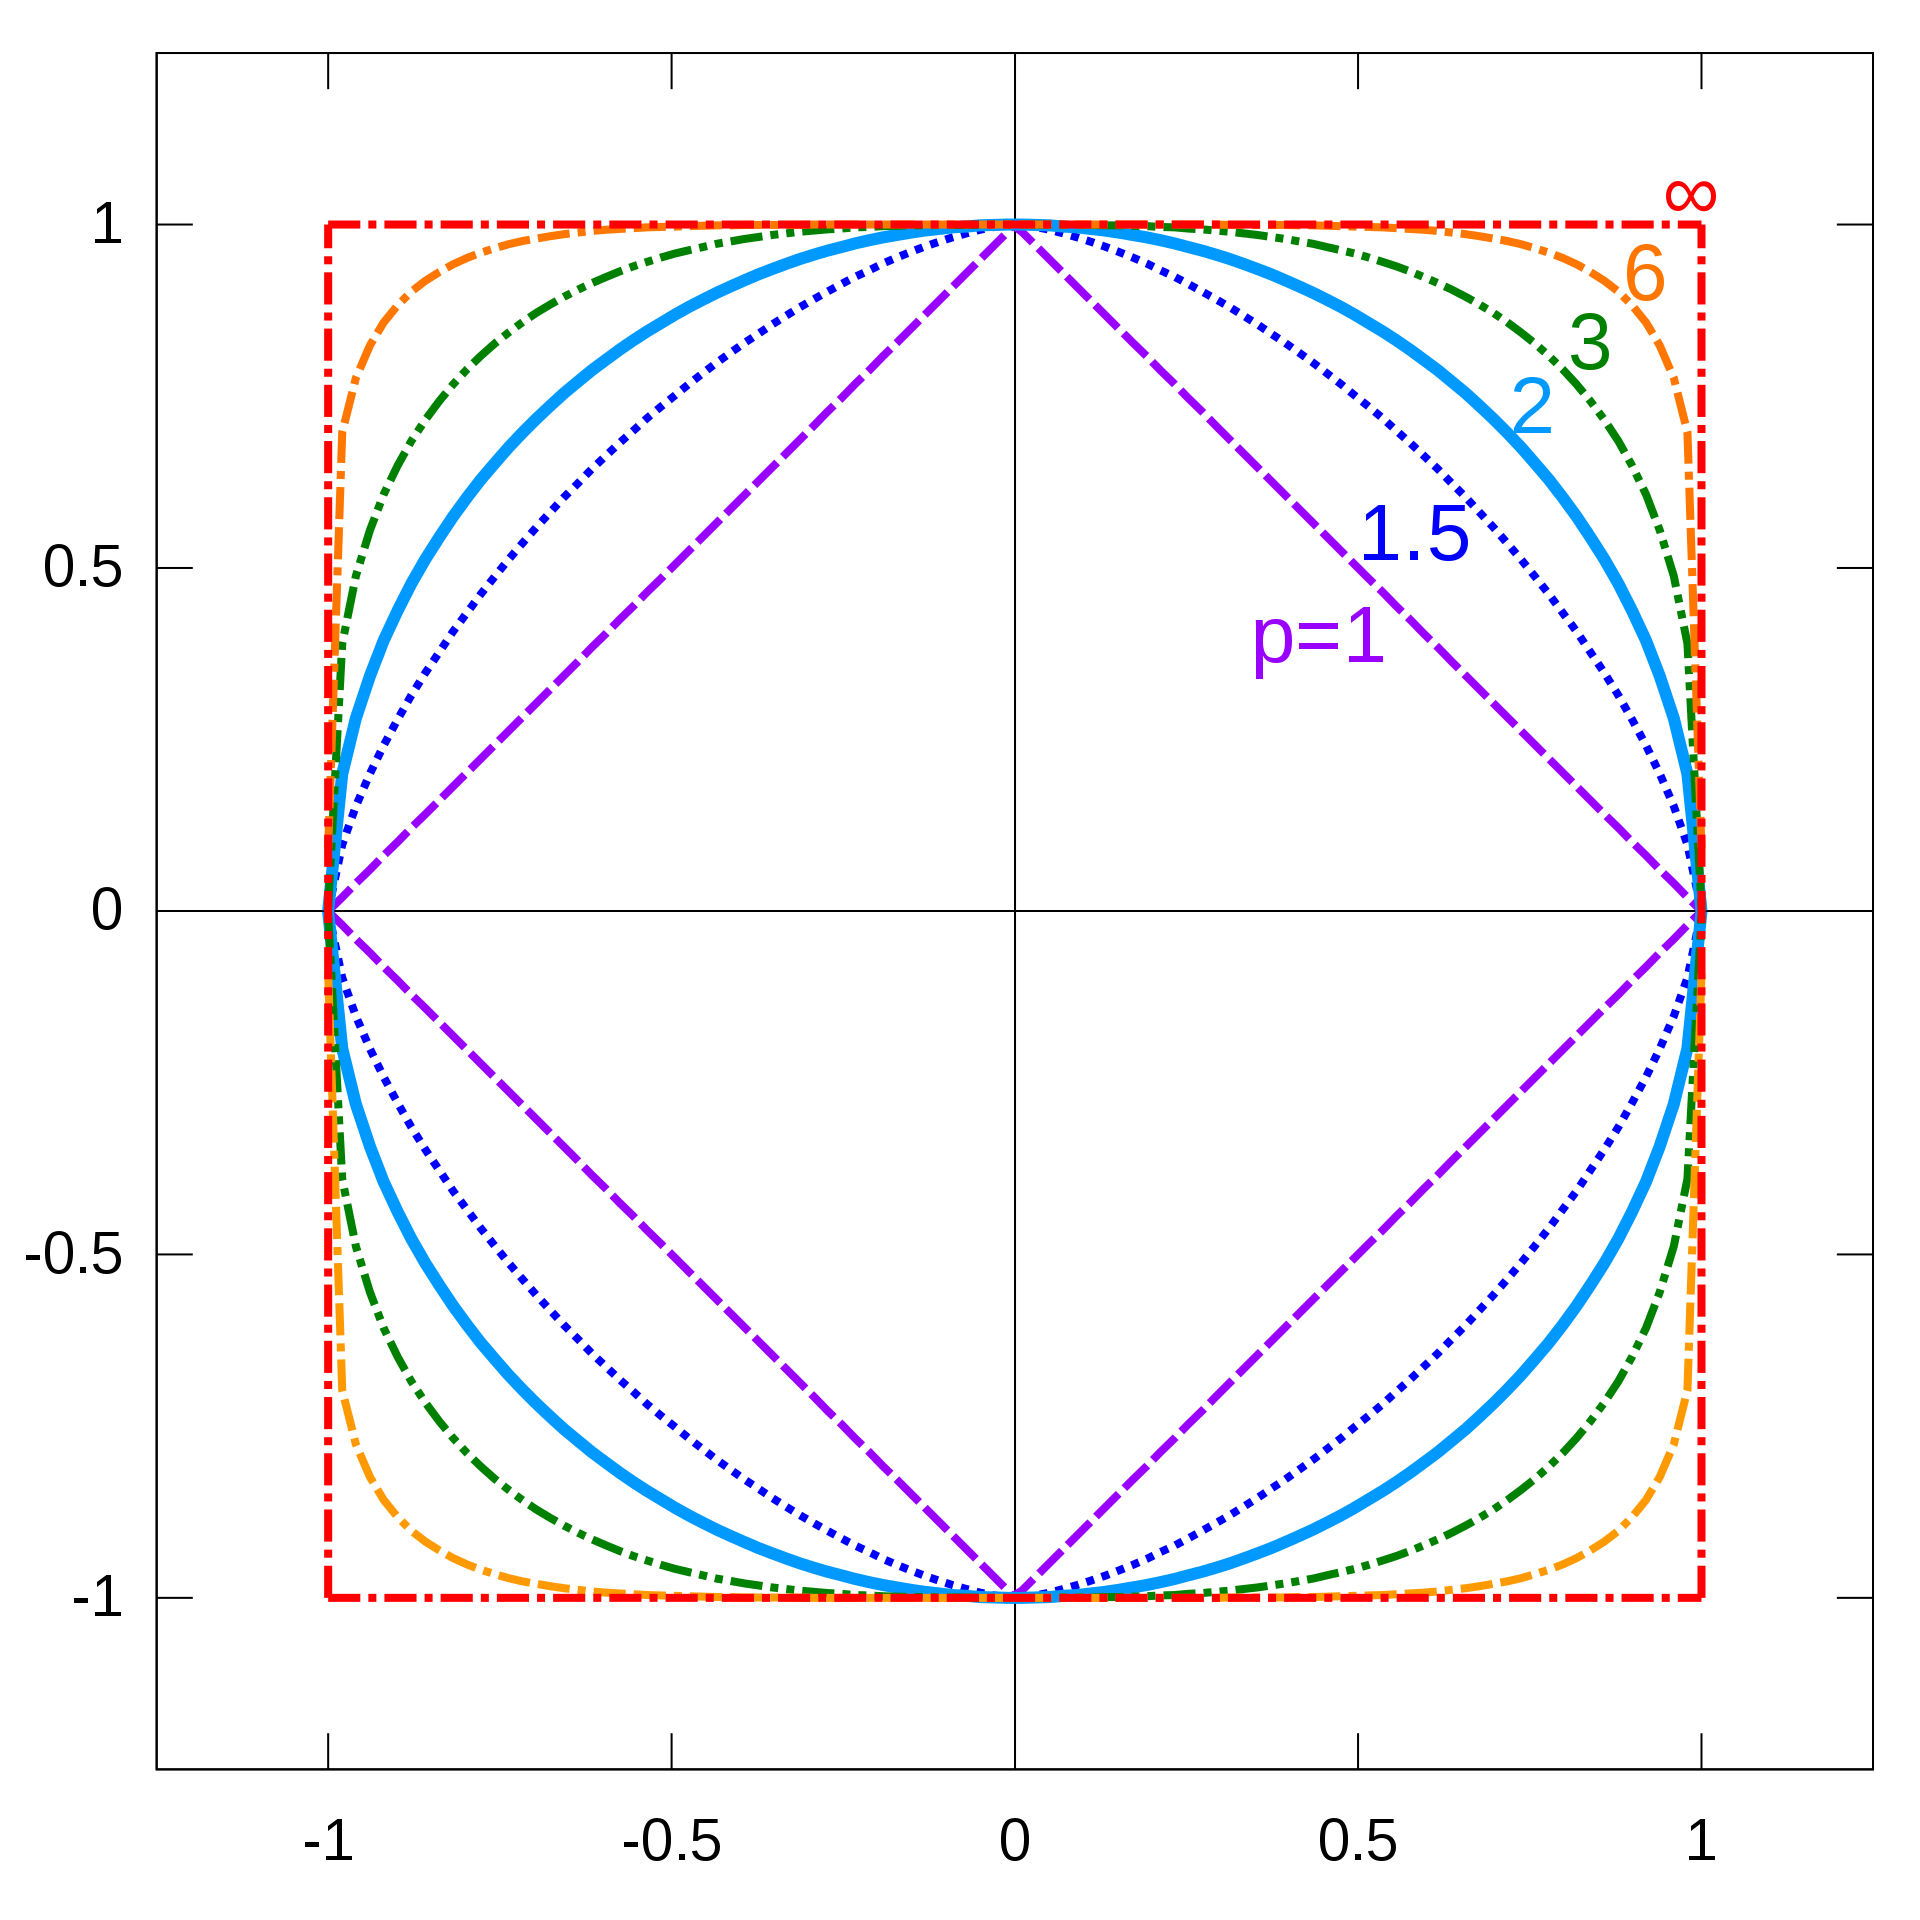
\includegraphics[scale = 0.1]{\pathtoimages/p-Norms.png}
\end{center}

\end{frame}

\begin{frame}
\frametitle{Inner Products Induce Norms}
If $V$ is an inner product space, the norm induced by the inner product is
$$
\| {\boldsymbol v}\| = \sqrt{\langle {\boldsymbol v}, {\boldsymbol v} \rangle}.
$$
\end{frame}

\begin{frame}[t]
\frametitle{Law of Cosines and Inner Products}
People like to think of inner products defining the angle $\theta$ between vectors
$$
\langle {\boldsymbol u}, {\boldsymbol v}\rangle = \| {\boldsymbol u}\| \|{\boldsymbol v}\|\cos\theta
$$
In particular, we say ${\boldsymbol u}$ and ${\boldsymbol v}$ are {\bf orthogonal} if
$$
\langle {\boldsymbol u}, {\boldsymbol v}\rangle = 0.
$$
\end{frame}


\begin{frame}
\frametitle{Distance}
\begin{Definition}
A bivariate function $d$ on a set $V$ is a {\bf distance metric} if for all ${\boldsymbol u}, {\boldsymbol v}, {\boldsymbol w}$ in $V$ the following hold.
\begin{enumerate}
\item[D.1] $d({\boldsymbol u}, {\boldsymbol v}) \geq 0$ and $d({\boldsymbol u}, {\boldsymbol v}) = 0$ if and only if ${\boldsymbol u} = {\boldsymbol v}$
\item[D.2] $d({\boldsymbol u}, {\boldsymbol v}) = d({\boldsymbol v}, {\boldsymbol u})$
\item[D.3]  $d({\boldsymbol u}, {\boldsymbol v}) + d({\boldsymbol v}, {\boldsymbol w}) \geq d({\boldsymbol u}, {\boldsymbol w})$
\end{enumerate}
\end{Definition}
\end{frame}

\begin{frame}
\frametitle{Distance Metric Examples}

\begin{itemize}
\item For the real vector space $\mathbb{R}^n$, the Euclidean distance is most common. Given ${\boldsymbol x} = \left(x_1, x_2, \ldots, x_n\right)$ and ${\boldsymbol y} = (y_1, y_2, \ldots, y_n)$, it is defined to be
$$
d({\boldsymbol x}, {\boldsymbol y})= \sqrt{(x_1 - y_1)^2 + (x_2 - y_2)^2 +\ldots + (x_n -y_n)^2}.
$$
\item The discrete metric on any set:
$$
d({\boldsymbol x}, {\boldsymbol y}) = \begin{cases} 1	&	{\boldsymbol x} \neq {\boldsymbol y} \\ 0	&	{\boldsymbol x} = {\boldsymbol y}.\end{cases}
$$
\item On the set of continuous real-valued functions on the interval [0, 1], we can define
$$
d(f, g) = \int_0^1 \left| f(x) - g(x)\right|\ dx.
$$
\end{itemize}

\end{frame}

\begin{frame}
\frametitle{Norms Induce Distances}
The distance metric induced by a norm is
$$
d({\boldsymbol u}, {\boldsymbol v}) = \| {\boldsymbol u} - {\boldsymbol v}\|.
$$
\end{frame}

\subsection{Projections}

\begin{frame}[t]
\frametitle{Projection}
The projection of ${\boldsymbol v}$ onto ${\boldsymbol u}$ is
$$
proj_{\boldsymbol u}({\boldsymbol v}) = \frac{\langle {\boldsymbol u}, {\boldsymbol v} \rangle}{\| {\boldsymbol u}\|^2} {\boldsymbol u}.
$$
\begin{figure}
\centering
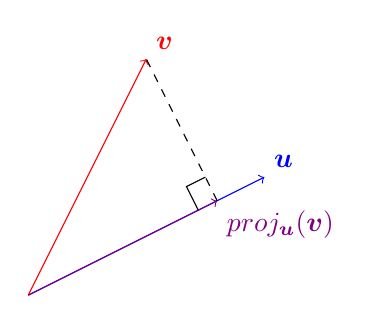
\begin{tikzpicture}[scale = 1.5]

\draw[->, color = blue] (0, 0) -- (2, 1) node[above right] {$\boldsymbol u$};
\draw[->, color = red] (0, 0) -- (1, 2) node[above right] {$\boldsymbol v$};
\draw[->, color = violet] (0, 0) -- (1.6, 0.8) node[below right] {$proj_{\boldsymbol u}({\boldsymbol v})$};

\draw[dashed] (1.6, 0.8) -- (1, 2);

\draw (1.44, 0.72) -- (1.34, 0.92) -- (1.5, 1.0);

\end{tikzpicture}
\end{figure}
\end{frame}



\begin{frame}[t]
\frametitle{Projection Example}

\begin{Example}
Suppose
$$
{\boldsymbol u} = \left(\begin{array}{c} 2\\ 1\end{array}\right)\qquad\text{and}\qquad {\boldsymbol v} = \left(\begin{array}{c} 1\\ 2\end{array}\right).
$$
Compute $proj_{\boldsymbol u}( {\boldsymbol v})$.
\end{Example}

\end{frame}

\begin{frame}[fragile]
\frametitle{Projection Solution Python Code}

\begin{multicols}{2}
\begin{lstlisting}[language=Python]
# Import modules
import numpy as np, matplotlib.pyplot as plt

# Use Seaborn style; use LaTeX
plt.style.use('seaborn')
plt.rcParams['text.usetex'] = True

# Define u and v
u, v = np.array([2, 1]), np.array([1, 2])

# Calculate projection; key step
proj = np.dot(u, v)/np.linalg.norm(u)**2 * u

# Calculate the part of v perpendicular to u
u_perp = v - proj

# Define origin
origin = np.array([0, 0])

# Plot figure
fig, ax = plt.subplots(1, 1, dpi = 150)

# Draw arrow for u
ax.arrow(*origin, *u, label = r'$\vec{u}$', 
	color = 'blue', width = 0.01, 
         length_includes_head = True)

# Draw arrow for v
ax.arrow(*origin, *v, label = r'$\vec{v}$', 
         color = 'red', width = 0.01, 
         
         
         length_includes_head = True)

# Draw arrow for projection
ax.arrow(*origin, *proj, label = r'$proj_{\vec{u}}(\vec{v})$', 
           	color = 'purple', width = 0.01, 
         	length_includes_head = True)

# Draw arrow for part of v perpendicular to u
# Place initial side at terminal side of projection
ax.arrow(*proj, *u_perp, label = r'$v - proj_{\vec{u}}(\vec{v})$', 
           color = 'gray', width = 0.01, 
         length_includes_head = True)

# Add a little horizontal space for legend
ax.set_xlim([0, np.max([u[0], v[0], proj[0], u_perp[0]]) + 0.2])

# Make aspect ratio equal
fig.gca().set_aspect('equal')

# Place legend at upper right
ax.legend(loc = 'upper right')

# Save the figure
plt.savefig(path + r'ex2-1.png')

# Show graph
plt.show()
\end{lstlisting}
\end{multicols}

\end{frame}

\begin{frame}[fragile]
\frametitle{Projection Result}
\begin{figure}
\centering
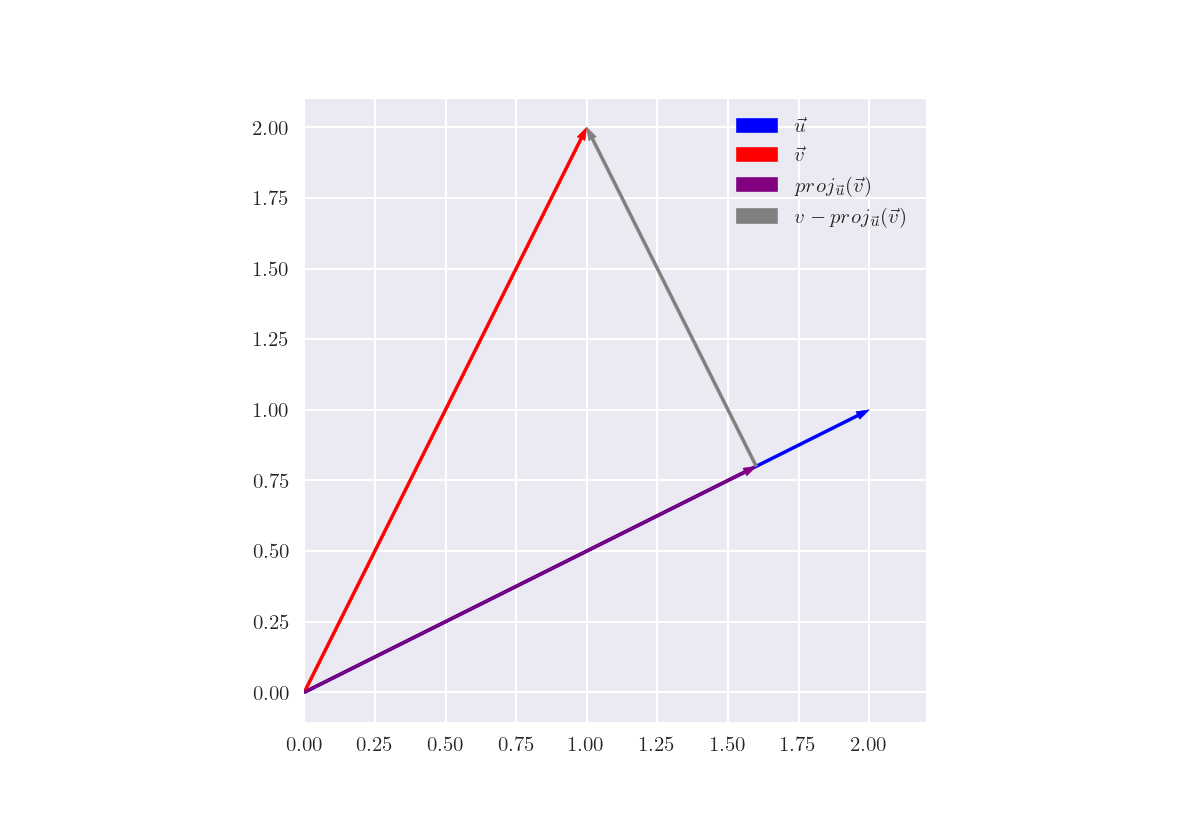
\includegraphics[scale = 0.5]{\pathtoimages/ex2-1.png}
\end{figure}
\end{frame}


\begin{frame}
\frametitle{Gram-Schmidt Orthogonalization Process}
\begin{Theorem}
If $({\boldsymbol v_1}, {\boldsymbol v_2}, \ldots, {\boldsymbol v_n})$ is a sequence of linearly independent vectors in an inner product space $V$, then the sequence $({\boldsymbol u_1}, {\boldsymbol u_2},\ldots, {\boldsymbol u_n})$, defined by
$$
{\boldsymbol u_1} = {\boldsymbol v_1}\qquad\text{and}\qquad {\boldsymbol u_k} = {\boldsymbol v_k} - \sum_{i = 1}^{k - 1} \frac{\langle {\boldsymbol v_k}, {\boldsymbol u_i}\rangle}{\| {\boldsymbol u_i}\|^2} {\boldsymbol u_i}
$$
for $k = 2, 3,\ldots, n$, is an orthogonal sequence in $V$ with the property that
$$
\text{span}\{{\boldsymbol u_1}, {\boldsymbol u_2},\ldots, {\boldsymbol u_n}\} = \text{span}\{{\boldsymbol v_1}, {\boldsymbol v_2},\ldots, {\boldsymbol v_n}\}.
$$
\end{Theorem}

\end{frame}

\begin{frame}[t]
\frametitle{Gram-Schmidt Orthogonalization Process}
\small
\begin{Example}
Orthogonalize the first two vectors of the basis $(1, x, x^2,\ldots)$ for the set of polynomials over $\mathbb{R}$ with inner product
$$
\langle p, q\rangle = \int_{0}^1 p(x)q(x)\ dx.
$$
\end{Example}


\end{frame}

\begin{frame}
\frametitle{Orthogonal Basis}
If $({\boldsymbol u_1}, {\boldsymbol u_2},\ldots, {\boldsymbol u_n})$ is an orthogonal basis of $V$, then for ${\boldsymbol v}$ in $V$ we have
$$
{\boldsymbol v} = \alpha_1 {\boldsymbol u_1} + \alpha_2 {\boldsymbol u_2} +\ldots + \alpha_n {\boldsymbol u_n}
$$ 
implies
$$
\alpha_i = \frac{\langle {\boldsymbol u_i}, {\boldsymbol v} \rangle}{\|{\boldsymbol u_i}\|^2}.
$$
\end{frame}

\begin{frame}
\frametitle{Cauchy-Schwarz Inequality}
\begin{Theorem}[Cauchy-Schwarz Inequality]
Suppose ${\boldsymbol u}$ and ${\boldsymbol v}$ are in the inner product space $V$. Then
$$
|\langle {\boldsymbol u}, {\boldsymbol v}\rangle| \leq \|{\boldsymbol u}\| \|{\boldsymbol v}\|.
$$
\end{Theorem}
\end{frame}

\begin{frame}
\frametitle{The Projection Theorem}
\begin{Definition}
The {\bf orthogonal complement} of a set $X\subseteq V$ is the set
$$
X^\perp = \{{\boldsymbol v} \in V| \langle {\boldsymbol x}, {\boldsymbol v}\rangle = 0\ \text{for all}\ {\boldsymbol x}\in X\}.
$$
\end{Definition}

\begin{Theorem}[Projection Theorem]
If $U$ is a finite-dimensional subspace of an inner product space $V$, then for each element ${\boldsymbol v}$ in $V$, there exists unique elements ${\boldsymbol u}$ in $U$ and ${\boldsymbol w}$ in $U^\perp$ such that ${\boldsymbol v} = {\boldsymbol u} + {\boldsymbol w}$.
\end{Theorem}
\end{frame}


\begin{frame}
\frametitle{Best Approximation}
The Projection Theorem tells us that for ${\boldsymbol u'}$ in $U$, we will alway have
$$
\| {\boldsymbol v} - {\boldsymbol u}\| \leq \| {\boldsymbol v} - {\boldsymbol u'}\|,
$$
where
$$
proj_U({\boldsymbol v})= {\boldsymbol u }.
$$

\end{frame}

\begin{frame}[t]
\frametitle{Easy Projection Example}
\begin{Example}
Consider the subspace $U$ of $\mathbb{R}^3$ spanned by the orthogonal vectors 
$$
{\boldsymbol u_1} = \left(\begin{array}{c} 1\\ 1\\ 0\end{array}\right)\qquad\text{and}\qquad {\boldsymbol u_2} = \left(\begin{array}{c} 1\\ -1\\ 0\end{array}\right).
$$
Compute the best approximation of ${\boldsymbol v} =(1, 2, 3)^T$ contained in $U$.
\end{Example}
\end{frame}

\begin{frame}[fragile]
\frametitle{Easy Projection Python Code}
\begin{lstlisting}[language=Python]
import numpy as np

# Define u1 and u2
u1, u2 = np.array([1, 1, 0]), np.array([1, -1, 0])

# Define v
v = np.array([1, 2, 3])

# Calculate projection

# First, projection onto u1
proj = np.dot(u1, v)/np.linalg.norm(u1)**2 * u1 

# Second, add projection onto u2
proj += np.dot(u2, v)/np.linalg.norm(u2)**2 * u2

proj
\end{lstlisting}
The result is [1, 2, 0] as expected.
\end{frame}

\begin{frame}[t]
\frametitle{Projection Check}
\begin{Example}
Consider the subspace $U$ of $\mathbb{R}^3$ spanned by the orthogonal vectors 
$$
{\boldsymbol u_1} = \left(\begin{array}{c} 1\\ 1\\ 0\end{array}\right)\qquad\text{and}\qquad {\boldsymbol u_2} = \left(\begin{array}{c} 1\\ -1\\ 0\end{array}\right),
$$
and ${\boldsymbol v} =(1, 2, 3)^T$. Randomly generate elements ${\boldsymbol u'}$ in U to verify that  $\| {\boldsymbol v} - proj_U({\boldsymbol v})\| \leq \| {\boldsymbol v} - {\boldsymbol u'}\|$.
\end{Example}
\end{frame}

\begin{frame}[fragile]
\frametitle{Projection Check Python Code}
\begin{lstlisting}[language=Python]
# Calculate minimal norm
min_norm = np.linalg.norm(v - proj)

# Define number of trials
trials = 100_000

# Initialize object to hold results
norm_vals = np.zeros(trials)

for i in range(trials):
    
    # Generate weights; use guassian distribution
    alpha = np.random.normal(size = 2)
    
    # Calculate u'
    u_prime = alpha[0] * u1 + alpha[1] * u2
    
    # Calculate and record norm
    norm_vals[i] = np.linalg.norm(v - u_prime)
    
print(f'The number of norms less than the norm of v - proj_U(v) is {np.sum(norm_vals < min_norm)}.')
\end{lstlisting}
The output reads:
\begin{quote}
\small
\texttt{The number of norms less than the norm of v - proj\_U(v) is 0.}
\end{quote}
This was the expected result!
\end{frame}

\begin{frame}[fragile]
\frametitle{Projection Check Histogram Python Code}

\begin{lstlisting}[language=Python]
import matplotlib.pyplot as plt

# Use Seaborn style
plt.style.use('seaborn')

# Use LaTeX
plt.rcParams['text.usetex'] = True

# Plot histogram
plt.hist(norm_vals, label = r"$\|\vec{v} - \vec{u}'\|$", bins = int(np.sqrt(trials)))

# Plot vertical line
plt.axvline(min_norm, ymin = 0, ymax = 1, label = r'$\| \vec{v} - proj_U(\vec{v})\|$', 
           color = 'red')

# Give plot a title
plt.title(r"$\min_{\vec{u}'\in U} \| \vec{v} - \vec{u}'\| = $ " + f'{np.min(norm_vals):.5f};' +
             r' $\|\vec{v} - proj_{U}(\vec{v})\| = $ ' + f'{min_norm:.5f}.', fontsize = 15)

# Create a legend
plt.legend(fontsize = 12)

# Save the figure
plt.savefig(path + r'ex2-2.png')

plt.show()
\end{lstlisting}
\end{frame}

\begin{frame}[fragile]
\frametitle{Projection Check Histogram}
\begin{center}
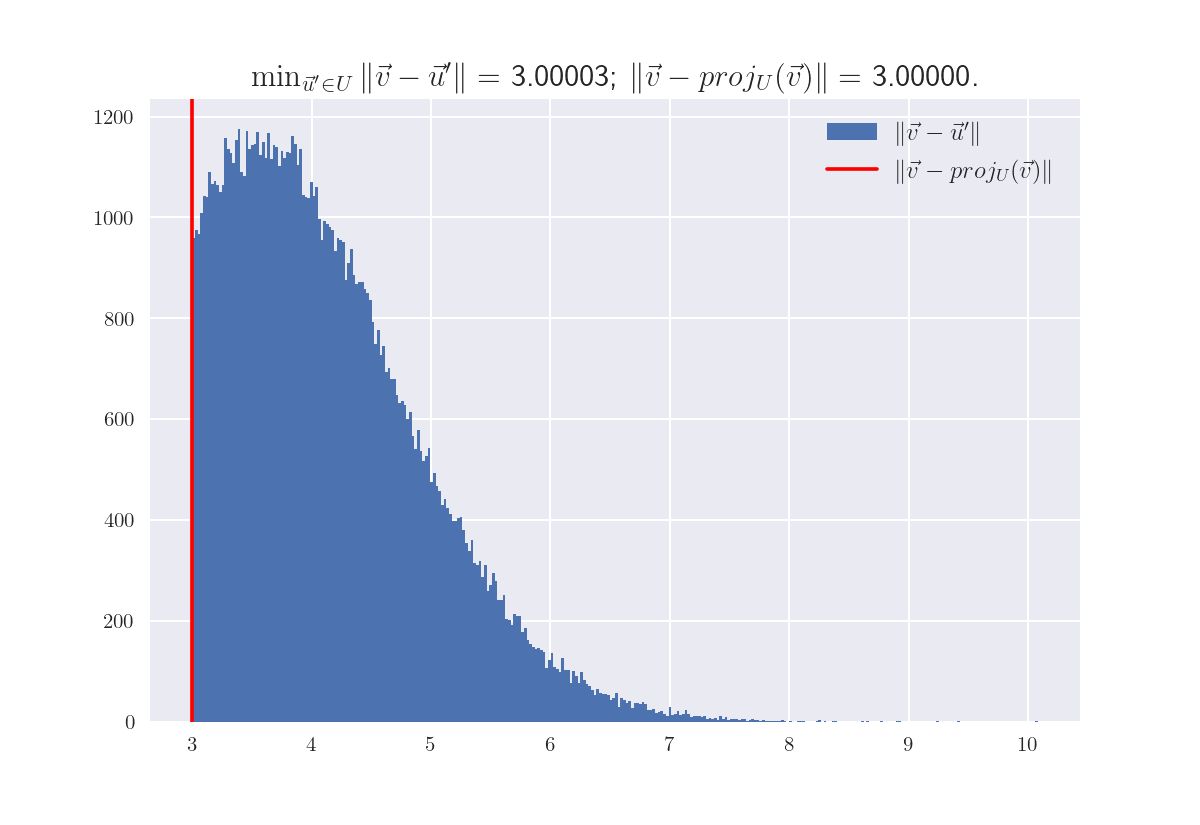
\includegraphics[scale = 0.5]{\pathtoimages/ex2-2.png}
\end{center}
\end{frame}

\begin{frame}[t]
\frametitle{Hard Projection Example}
\begin{Example}
Consider the inner product space of continuous functions on $[0, 1]$, where the inner product is
$$
\langle p, q\rangle = \int_0^1 p(x) q(x)\ dx.
$$
Project $e^x$ onto the subspace spanned by the orthogonal vectors $1$ and $x - 1/2$. Compare the projection with the tangent line approximation at $x = 1/2$.
\end{Example}
\end{frame}

\begin{frame}
\frametitle{Hard Projection Example Solution}
 {\tiny  {\bf Solution.} The projection is
$$
proj(x) = a_{proj}+ b_{proj} \left(x - \frac{1}{2}\right),
$$
where
\begin{align*}
a_{proj}	& = \frac{\langle 1, e^x\rangle}{\|1\|^2}		&	b_{proj} 	&= \frac{\langle x - 1/2, e^x\rangle}{\| x - 1/2 \|^2}\\
		& = \frac{\int_0^1 e^x\ dx}{\int_0^1 1^2\ dx}	&			&= \frac{ \int_0^1 (x - 1/2)e^x\ dx}{\int_0^1 (x - 1/2)^2\ dx} \\
		& = e - 1								&			&=  6(3 - e).
\end{align*}
The tangent line approximation is
$$
tan\_line(x) = a_{tl} + b_{tl} \left(x - \frac{1}{2}\right),
$$
where
$$
a_{tl} = e^{1/2}\qquad b_{tl} = e^{1/2}.
$$
}

\end{frame}

\begin{frame}[fragile]
\frametitle{Hard Projection Example Solution Python Code}
\begin{lstlisting}[language=Python]
# Import numerical integrator
from scipy.integrate import quad

# Define inner product
inner = lambda f, g: quad(lambda x: f(x) * g(x), 0, 1)[0]

# Define basis elements
u1, u2 = lambda x: 1, lambda x: x - 1/2 

# Calculate inner products
a_proj, b_proj = inner(u1, np.exp)/inner(u1, u1), inner(u2, np.exp)/inner(u2, u2) 

# Define small value
h = 1e-5

# Calculate tangent line coeffs
a_tl, b_tl = np.exp(0.5), (np.exp(0.5 + h) - np.exp(0.5 - h))/(2 * h)

# Define functions 
proj = lambda x: a_proj * u1(x) + b_proj * u2(x)
tan_line = lambda x: a_tl * u1(x) + b_tl * u2(x)

# Get the x-values for plot
x_vals = np.linspace(0, 1, 100)

# Plot results
plt.plot(x_vals, proj(x_vals), label = 'Projection')
plt.plot(x_vals, tan_line(x_vals), label = 'Tangent Line')
plt.plot(x_vals, np.exp(x_vals), label = 'True')

# Create a legend
plt.legend()

# Save the figure and show figure
plt.savefig(path + r'ex2-3.png')
plt.show()
\end{lstlisting}
\end{frame}

\begin{frame}[fragile]
\frametitle{Hard Projection Example Image}
\begin{center}
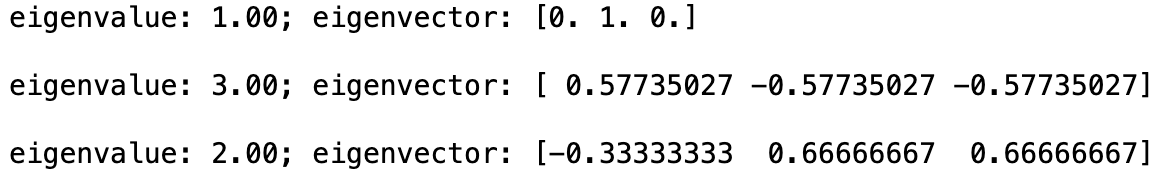
\includegraphics[scale = 0.5]{\pathtoimages/ex2-3.png}
\end{center}
\end{frame}

\begin{frame}[fragile]
\frametitle{Projection Example Result}

\begin{lstlisting}[language=Python]
# Define norm
norm = lambda f: np.sqrt(inner(f, f))

# Let's calculate the norms
norm_proj, norm_tl = norm(lambda x: np.exp(x) - proj(x)), norm(lambda x: np.exp(x) - tan_line(x))

print(f'Using the projection approximation the norm is {norm_proj:.3f}.')
print(f'Using the tangent line approximation the norm is {norm_tl:.3f}.')
\end{lstlisting}
The output reads:
\begin{quote}
{
\small
\texttt{Using the projection approximation the norm is 0.063.}\\
\texttt{Using the tangent line approximation the norm is 0.094.}
}
\end{quote}
\end{frame}


\subsection{Determinants}

\begin{frame}
\frametitle{Determinant of a $ 2\times 2$ Matrix}
Suppose 
$$
A = \left(\begin{array}{c c} a	&	b\\ c	& d\end{array}\right).
$$
Then
$$
\text{det}(A) = \left| \begin{array}{c c} a	&	b\\ c	& d\end{array}\right| = ad - bc.
$$
\end{frame}

\begin{frame}[t]
\frametitle{Determinant Example}
\begin{Example}
$\left|\begin{array}{c c} -1	&	-5\\	2	&	1\end{array}\right|=$
\end{Example}

\end{frame}

\begin{frame}
\frametitle{Determinant of an $n\times n$ Matrix}
Suppose $A$ is the $n\times n$ matrix
$$
A = \left(a_{ij} \right).
$$
Let $A_{ij}$ denote $A$ with the $i$-th row and $j$-th column removed. Then
$$
\text{det}(A) = \sum_{j = 1}^n (-1)^{i + j} a_{ij}\text{det}(A_{ij})
$$
for any choice of $i$ in $\{1, 2,\ldots, n\}$.

\end{frame}

\begin{frame}[t]
\frametitle{Determinant Example}
\begin{Example}
$
\left|\begin{array}{c c c} 2	&	1	&	2\\	0	&	3	&	-1\\	4	&	1	&	1\end{array}\right| = 
$
\end{Example}

\end{frame}

\begin{frame}
\frametitle{Properties of Determinants} 
{\tiny
Let $A$ and $B$ be $n\times n$ matrices, ${\boldsymbol a_j}$, ${\boldsymbol b}$, and ${\boldsymbol c}$ be $n\times 1$ vectors, and $\alpha$ and $\beta$ real numbers.
\begin{enumerate}
\item[(a)] If the columns of $A$ are linearly dependent, $\text{det}(A) = 0$.
\item[(b)] If $A^{-1}$ exists, then $\text{det}(A^{-1}) = \frac{1}{\text{det}(A)}$.
\item[(c)] $\text{det}(\alpha A) = \alpha^n \text{det}(A)$.
\item[(d)] $\text{det}(A^T) = \text{det}(A)$
\item[(e)] $\text{det}(AB) = \text{det}(A)\text{det}(B)$
\item[(f)]  $\text{det}(I) = 1$

\item[(g)] $
\left| {\boldsymbol a_1}\;	{\boldsymbol a_2}\; \ldots {\boldsymbol a_{j - 1}}\;	\alpha {\boldsymbol b}  + \beta {\boldsymbol c}\; {\boldsymbol a_{j + 1}}  \ldots\;  {\boldsymbol a_n}\right| = \alpha \left| {\boldsymbol a_1}\; {\boldsymbol a_2}\; \ldots {\boldsymbol a_{j - 1}}\; {\boldsymbol b}\; {\boldsymbol a_{j + 1}} \ldots  {\boldsymbol a_n}\right| + \beta \left| {\boldsymbol a_1}\; {\boldsymbol a_2}\;	 \ldots {\boldsymbol a_{j-1}}\; {\boldsymbol c} \; {\boldsymbol a_{j + 1}} \ldots {\boldsymbol a_n}\right|.
$
\item[(h)] $
\left| {\boldsymbol a_1}\;	{\boldsymbol a_2}\; \ldots {\boldsymbol a_{j }}\;	{\boldsymbol a_{j + 1}}   \ldots\;  {\boldsymbol a_n}\right|  = -\left| {\boldsymbol a_1}\;	{\boldsymbol a_2}\; \ldots {\boldsymbol a_{j + 1}}\;	{\boldsymbol a_{j}}   \ldots\;  {\boldsymbol a_n}\right| 
$
\end{enumerate}
Property (a) is very important. In \texttt{numpy}, there's \texttt{np.linalg.det} which computes the determinant. Since computers will be available to you in most circumstances the other properties are less important.}
\end{frame}

\subsection{Cramer's Rule}

\begin{frame}
\frametitle{Cramer's Rule}
\small
Consider a system of $n$ linear equations with $n$ unknowns
$$
 A {\boldsymbol x} = {\boldsymbol b}
$$
where $A$ is an $n\times n$ matrix with nonzero determinant and 
$$
{\boldsymbol x} = \left(\begin{array}{c} x_1\\ x_2\\ \vdots\\ x_n\end{array}\right).
$$
Then 
$$
x_i = \frac{\text{det}(A_i)}{\text{det}(A)},
$$
where $A_i$ is the matrix formed by replacing the $i$-th column of $A$ by the column vector ${\boldsymbol b}$.
\end{frame}

\begin{frame}[t]
\frametitle{Cramer's Rule Example}
\small
\begin{Example}
Solve the system 
$$
\begin{array}{r c c l}
3x 	&+ 2y 	&- 2z 	&= 1\\
2x 	&- y		&		&= 0\\
	&-4y 		&+ 3z	&= 1.
\end{array} 		
$$
\end{Example}


\end{frame}



\subsection{Eigenvectors and Eigenvalues}

\begin{frame}
\frametitle{Eigenvectors and Eigenvalues}
\begin{Definition}
Let $V$ be a vector space and consider a linear transformation $T:V\to V$ with matrix representation $A$. An element ${\boldsymbol v}$ in $V$ is an {\bf eigenvector} of $A$ if there exists a number $\lambda$ such that $A{\boldsymbol v} = \lambda {\boldsymbol v}$. If ${\boldsymbol v}\neq {\boldsymbol 0}$, then $\lambda$ is called an {\bf eigenvalue} of $A$.
\end{Definition}
In \texttt{numpy}, we have \texttt{np.linalg.eig}. The function computes the eigenvalues and eigenvectors, respectively.
\end{frame}

\begin{frame}[t]
\frametitle{Eigenvector and Eigenvalues}
\begin{Example}
{\small
Let $A = \left(\begin{array}{c c} 1	&	1\\	1	&	1\end{array}\right)$. Show that ${\boldsymbol v_1} = \left(\begin{array}{c} 1\\	-1\end{array}\right)$ and ${\boldsymbol v_2} = \left(\begin{array}{c} 1\\ 1\end{array}\right)$ are eigenvectors. What are their eigenvalues?
}
\end{Example}

\end{frame}

\begin{frame}
\frametitle{Eigenvectors and Kernels}
If ${\boldsymbol v}$ is an eigenvector of $A$ with eigenvalue $\lambda$, then
$$
A{\boldsymbol v} = \lambda {\boldsymbol v}\qquad\text{implies}\qquad (A - \lambda I){\boldsymbol v} = {\boldsymbol 0}.
$$
So, if ${\boldsymbol v}\neq {\boldsymbol 0}$, then $\text{Ker}(A - \lambda I) \neq \{{\boldsymbol 0}\}$. This, implies $A - \lambda I$ has linearly dependent columns. Hence, $\text{det}(A - \lambda I) = 0$.

\end{frame}

\begin{frame}

\begin{Definition}
\frametitle{Characteristic Polynomial}
For an $n\times n$ matrix $A$, the {\bf characteristic polynomial} of $A$ is
$$
p_A(\lambda) = \text{det}(A - \lambda I).
$$
\end{Definition}
We can find the eigenvalues by finding the zeros of $p_A$. We can then plug the eigenvalues into $(A - \lambda I){\boldsymbol x} = {\boldsymbol 0}$ to find the corresponding eigenvectors.
\end{frame}

\begin{frame}[t]
\frametitle{Using the Characteristic Polynomial}
\begin{Example}
Find the eigenvalues and eigenvectors of $A = \left(\begin{array}{c c} 1	&	0.5\\ 0.5	&	1\end{array}\right)$.
\end{Example}

\end{frame}

\begin{frame}
\frametitle{Diagonalizable Matrices}
\begin{Definition}
We say that a matrix $A$ is {\bf diagonalizable} if $V$ has a basis of eigenvectors of $A$.
\end{Definition}
\end{frame}

\begin{frame}
\frametitle{Diagonalizable Matrices Example}
{
\tiny
In our previous example, we saw the eigenvectors of 
$$
A = \left(\begin{array}{c c} 1	&	0.5\\	0.5	&	1\end{array}\right),
$$
are
$$
{\boldsymbol v_1} = \left(\begin{array}{c} 1\\	-1\end{array}\right)\qquad\text{and}\qquad {\boldsymbol v_2} = \left(\begin{array}{c} 1\\ 1\end{array}\right).
$$  
These eigenvectors are linearly independent, so they form a basis for $\mathbb{R}^2$. As a result, $A$ is diagonalizable. In particular, we can use the basis $({\boldsymbol v_1}, {\boldsymbol v_2})$ for $\mathbb{R}^2$ and the change of basis formula to diagonalize $A$. Under the basis, $({\boldsymbol v_1}, {\boldsymbol v_2})$ the matrix representation of the linear transformation corresponding to $A$ is
$$
N^{-1}  A N= \left(\begin{array}{c c} 0.5	&	0\\	0	&	1.5\end{array}\right),
$$
where $N$ is the matrix which contains the basis elements $({\boldsymbol v_1}, {\boldsymbol v_2})$ as columns, i.e.
$$
N =  \left(\begin{array}{c c} 1	&	1\\ -1 & 1\end{array}\right) 
$$
Recall: ${\boldsymbol v_1}$ has eigenvalue 0.5 and ${\boldsymbol v_2}$ has eigenvalue $1.5$.
}
\end{frame}



\begin{frame}[t]
\frametitle{Eigenvectors and Eigenvalues Example}
\begin{Example}
Suppose $A = \left(\begin{array}{c c} 1	&	2\\	3	&	2\end{array}\right)$. Find a basis of eigenvectors as well as their eigenvalues.
\end{Example}

\end{frame}


\begin{frame}[fragile]
\frametitle{Eigenvectors and Eigenvalues Python Example}
\begin{Example}
Suppose $A = \left(\begin{array}{c c c} 4	&	0	&	1\\	-2	&1	&	0\\	-2	&	0	& 1\end{array}\right)$. Find a basis of eigenvectors as well as their eigenvalues.
\end{Example}
\end{frame}

\begin{frame}[fragile]
\frametitle{Eigenvectors and Eigenvalues Python Code and Result}

\begin{lstlisting}[language=Python]
import numpy as np

# Define matrix 
A = np.array([[4, 0, 1], [-2, 1, 0], [-2, 0, 1]])

# Get the eigenvalues and eigenvectors
evals, evecs = np.linalg.eig(A)

# Loop through results
for i in range(len(evals)):
    
    print(f'eigenvalue: {evals[i]:.2f}; eigenvector: {evecs[:, i]}\n')
 \end{lstlisting}

The output is shown below:
\begin{figure}
\centering

\includegraphics[scale = 0.5]{\pathtoimages/ex2-4.png}
\end{figure}
\end{frame}

\begin{frame}
\frametitle{Symmetric Matrices}
\begin{Definition}
Suppose $V$ is an inner product space, and $T:V\to V$. Then $T$ is {\bf symmetric} if we have the relation
$$
\langle T{\boldsymbol v}, {\boldsymbol w}\rangle = \langle {\boldsymbol v}, T{\boldsymbol w}\rangle
$$
for all ${\boldsymbol v}$ and ${\boldsymbol w}$ in $V$. 
\end{Definition}
For the dot product on $\mathbb{R}^n$, if $T$ has matrix representation $A$ then symmetric means $A = A^T$.
\end{frame}

\begin{frame}
\frametitle{Spectral Theorem}

\begin{Theorem}[Spectral Theorem]
Let $V$ be a finite dimensional non-trivial inner product space over the real numbers, and suppose $T:V\to V$ is a symmetric linear transformation with matrix representation $A$. Then $V$ has an orthogonal basis consisting of eigenvectors of $A$.
\end{Theorem}


\end{frame}

\begin{frame}
\frametitle{Linear Algebra on YouTube}
\small
Watch the 3Blue1Brown linear algebra video series. The series includes most of what has been covered here as well as other great material ({\small \url{https://www.youtube.com/playlist?list=PLZHQObOWTQDPD3MizzM2xVFitgF8hE_ab}}).
\begin{center}

\includegraphics[scale = 0.2]{\pathtoimages/3Blue1Brown_lin_alg.png}
\end{center}
\end{frame}

\section{Multivariable Calculus}
\begin{frame}
\begin{center}
\Huge Multivariable Calculus
\end{center}
\end{frame}


\subsection{Partial Derivatives}

\begin{frame}
\frametitle{Partial Derivatives}
{\small 
\begin{Definition}
Suppose we have $f:\mathbb{R}^n \to \mathbb{R}$. Then the {\bf partial derivative} of $f$ with respect to $x_i$ is
$$
\frac{\partial f}{\partial x_i} = \lim_{h\to 0} \frac{f(x_1, x_2,\ldots, x_i + h,\ldots, x_n) - f(x_1, x_2,\ldots, x_i,\ldots, x_n)}{h}.
$$
\end{Definition}
The most common case is $f:\mathbb{R}^2\to \mathbb{R}$ and $z = f(x, y)$. Then the two partials are
$$
f_x(x, y) = \frac{\partial z}{\partial x} = \lim_{h\to 0 } \frac{f(x + h, y) - f(x, y)}{h}
$$
and
$$
f_y(x, y) = \frac{\partial z}{\partial y} = \lim_{h\to 0 } \frac{f(x, y + h) - f(x, y)}{h}.
$$

}
\end{frame}

\begin{frame}
\frametitle{Clairaut's Theorem}

\begin{Theorem}[Clairaut]
Suppose $f$ is defined on a disk $D$ that contains the point $(a, b)$. If the functions $f_{xy}$ and $f_{yx}$ are both continuous on $D$, then
$$
f_{xy}(a, b) = f_{yx}(a, b).
$$
\end{Theorem}

\end{frame}

\begin{frame}
\frametitle{Difference Approximation}

\begin{Theorem}
Suppose $f_x$ and $f_y$ exist on a rectangular region $R$ with sides parallel to the axes and containing the points $(a, b)$ and $(a + \Delta x, b + \Delta y)$. Suppose $f_x$ and $f_y$ are continuous at the point $(a, b)$, and let
$$
\Delta z = f(a + \Delta x, b + \Delta y) - f(a, b).
$$
Then
$$
\Delta z = f_x(a, b)\Delta x + f_y(a, b)\Delta y + \varepsilon_1\Delta x + \varepsilon_2\Delta y
$$
where $\varepsilon_1,\varepsilon_2\to 0$ as $\Delta x,\Delta y\to 0$.

\end{Theorem}

\end{frame}

\begin{frame}[t]
\frametitle{Example}
\begin{Example}
Suppose $f(x, y, z) = \sqrt{xyz}$. Approximate $f(3.9, 4.2, 3.8)$.
\end{Example}

\end{frame}

\begin{frame}
\frametitle{The Chain Rule}

Suppose $u$ is a differentiable function of $n$ variables $x_1, x_2,\ldots, x_n$ and each $x_j$ is a function of the $m$ variables $t_1, t_2,\ldots, t_m$ such that the partial derivative $\frac{\partial x_j}{\partial t_i}$ exists each for all $i$ and $j$. Then $u$ is a function of $t_1, t_2,\ldots, t_m$ and
$$
\frac{\partial u}{\partial t_i} = \frac{\partial u}{\partial x_1}\frac{\partial x_1}{\partial t_i} + \frac{\partial u}{\partial x_2}\frac{\partial x_2}{\partial t_i} + \ldots + \frac{\partial u}{\partial x_n}\frac{\partial x_n}{\partial t_i}
$$
for any $i$.

\end{frame}

\begin{frame}[t]
\frametitle{Chain Rule Example}
\begin{Example}
Consider the Black-Scholes differential equation
$$
\frac{\partial V}{\partial t} + \frac{\sigma^2}{2} S^2 \frac{\partial^2 V}{\partial S^2} + r S \frac{\partial V}{\partial S} = r V.
$$
Rewrite the partial differential equation using the substitution $z = \ln S$.
\end{Example}

\end{frame}

\begin{frame}
\frametitle{Implicit Differentiation}
Suppose that $F(x, y) = 0$ and $y = f(x)$. Then
$$
\frac{\partial F}{\partial x} + \frac{\partial F}{\partial y} \frac{d y}{d x} = 0.
$$
So,
$$
\frac{dy}{dx} = -\frac{\frac{\partial F}{\partial x}}{\frac{\partial F}{\partial y}}= - \frac{F_x}{F_y}
$$
as long as $\frac{\partial F}{\partial x}$ is continuous and $\frac{\partial F}{\partial y}$ is both continuous and nonzero.
\end{frame}

\begin{frame}[t]
\frametitle{Implicit Differentiation Example}
\begin{Example}
Find $\frac{dy}{dx}$ if $x^3 + y^3 = 6xy$.
\end{Example}
\end{frame}

\begin{frame}
\frametitle{Gradient Vector}
Let's introduce new notation. Suppose $x\in\mathbb{R}^n$. Define
$$
\nabla f(x) = \left(\frac{\partial f}{\partial x_1}, \frac{\partial f}{\partial x_2},\ldots, \frac{\partial f}{\partial x_n}\right).
$$
\end{frame}

\subsection{Gradient Vectors}
\begin{frame}
\frametitle{Space Curve}
A curve in $\mathbb{R}^n$ can be defined in terms of a vector valued function ${\boldsymbol r}$, where ${\boldsymbol r}:I\to\mathbb{R}^n$ and $I$ is some subset of $\mathbb{R}$. 

For example, consider ${\boldsymbol r}:[0, 2\pi)\to\mathbb{R}^2$ such that ${\boldsymbol r}: t \mapsto \left(\cos t, \sin t\right)$. This defines a circle oriented counterclockwise in $\mathbb{R}^2$.
\begin{center}
\begin{tikzpicture}[scale = 1.5]
\draw[->] (-1.25, 0) -- (1.7, 0) node[right] {$x$};
\draw[->] (0, -1.25) -- (0, 1.25) node[above] {$y$};

\draw[blue] (0, 0) circle (1);


\node[blue] at (1,0) {.};
\node[blue] at (0,1) {.};
\node[blue] at (-1,0) {.};
\node[blue] at (0,-1) {.};
	
\draw[->, blue] (1, 0) -- (1, 0.1) node[right] {$t = 0$};
\draw[->, blue] (0, 1) -- (-0.1, 1) node[above left] {$t = \frac{\pi}{2}$};
\draw[->, blue] (-1, 0) -- (-1, -0.1) node[below left] {$t = \pi$};
\draw[->, blue] (0, -1) -- (0.1, -1) node[below right] {$t = \frac{3\pi}{2}$};

\end{tikzpicture}

\end{center}
\end{frame} 

\begin{frame}[t]
\frametitle{Derivatives of Space Curves}
The derivative of ${\boldsymbol r}:I\to\mathbb{R}^n$ is defined to be
$$
{\boldsymbol r }'(t) =\lim_{h\to 0} \frac{{\boldsymbol r}(t + h) - {\boldsymbol r}(t)}{h}.
$$
The derivative is tangent to the curve described by ${\boldsymbol r}$.
\begin{center}
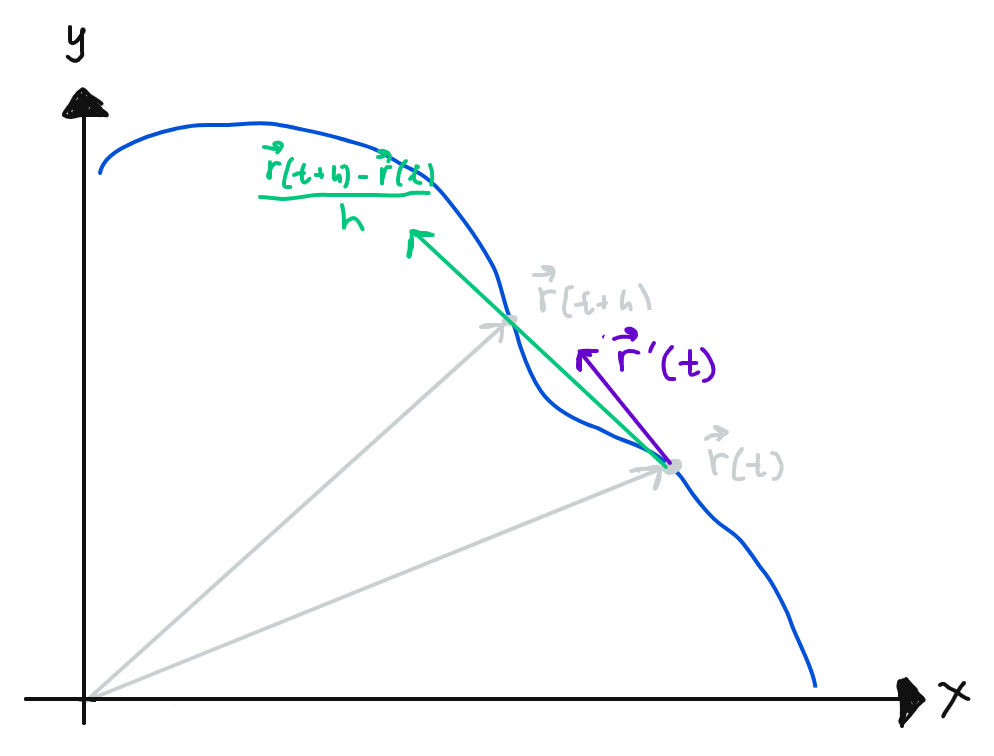
\includegraphics[scale = 0.25]{\pathtoimages/tangent.png}
\end{center}


\end{frame}

\begin{frame}
\frametitle{Gradient Vector Orthogonal to Surface}
\small 
Suppose that we have a surface defined by $F({\boldsymbol x}) = k$ where ${\boldsymbol x}$ is in $\mathbb{R}^n$. Consider any curve defined by ${\boldsymbol r}: I\to \mathbb{R}^n$. Then we have the value of the function at ${\boldsymbol r}(t)$ is
$$
F({\boldsymbol r}(t)) = k.
$$
The chain rule implies
$$
\nabla F({\boldsymbol r}(t))\bullet {\boldsymbol r'}(t) = 0.
$$
The vector ${\boldsymbol r'}(t)$ is parallel to the surface. Hence, $\nabla F({\boldsymbol r}(t))$ is orthogonal. Since ${\boldsymbol r}$ was arbitrary, $\nabla F(x)$ must be orthogonal to $F(x) = k$.
\end{frame}

\begin{frame}
\frametitle{Gradient Vector Example}

Consider $F(x, y) = x + y = 1$. Then $ \nabla F = (1, 1)$. We can see this vector is orthogonal to our line (or ``surface" to use the more general term).
\begin{center}
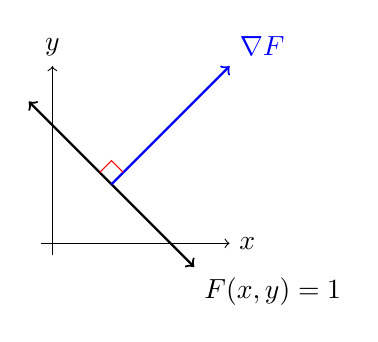
\begin{tikzpicture}[scale = 1.5]

\draw[->] (-0.1, 0) -- (1.5, 0) node[right] {$x$};
\draw[->] (0, -0.1) -- (0, 1.5) node[above] {$y$};

\draw[<->, thick] (-0.2, 1.2) -- (1.2, -0.2) node[below right] {$F(x, y) = 1$};

\draw[->, blue, thick] (0.5, 0.5) -- (1.5, 1.5) node[above right] {$\nabla F$};

\draw[red] (0.4, 0.6) -- (0.5, 0.7) -- (0.6, 0.6);
\end{tikzpicture}
\end{center}
\end{frame}


\subsection{Maximum and Minimum Values}

\begin{frame}
\frametitle{Local Maximum and Minimum}

\begin{Definition}
\begin{itemize}
\item A function of two variables has a {\bf local maximum} at $(a, b)$ if $f(x, y)\leq f(a, b)$ for all points $(x, y)$ in some disk with center $(a, b)$. The number $f(a, b)$ is called a {\bf local maximum value}. 
\item A function of two variables has a {\bf local minimum} at $(a, b)$ if $f(x, y)\geq f(a, b)$ for all points $(x, y)$ in some disk with center $(a, b)$. The number $f(a, b)$ is called a {\bf local minimum value}. 
\end{itemize}
\end{Definition}

\begin{Theorem}
If $f$ has a local extremum at $(a, b)$ and the first-order partial derivatives of $f$ exist there, then $f_x(a, b) = f_y(a, b) = 0$.
\end{Theorem}

\end{frame}


\begin{frame}
\frametitle{Second Derivatives Test}
Suppose the second partial derivatives of $f$ are continuous in a disk with center $(a, b)$, and suppose that $f_x(a, b) = f_y(a, b) = 0$. Let
$$
D = \left|\begin{array}{c c} f_{xx}(a, b)	&	f_{xy}(a, b)\\ f_{yx}(a, b)	&	f_{yy}(a, b)\end{array}\right|.
$$
\begin{enumerate}
\item[(a)] If $D >0$ and $f_{xx} (a, b) > 0$, then $f(a,b)$ is a local minimum.
\item[(b)] If $D > 0$ and $f_{xx}(a, b) < 0$, then $f(a, b)$ is a local maximum.
\item[(c)] If $D < 0$, then $f(a, b)$ is not a local extremum.
\item[(d)] If $D = 0$, then the test fails.
\end{enumerate}

\end{frame}


\begin{frame}[t]
\frametitle{Second Derivatives Test Example}
\begin{Example}
Find the shortest distance from the point $(1, 0, -2)$ to the plane $x + 2y + z = 4$.
\end{Example}
\end{frame}

\begin{frame}[fragile]
\frametitle{Minimization Python Example}
\small

\begin{Example}
Use Python to verify the previous example.
\end{Example}

\begin{lstlisting}[language=Python]
import numpy as np
from scipy.optimize import minimize

# Define function
def distance(pt):
    
    # Get the x- and y-values
    x, y = pt[0], pt[1]
    
    # Define z 
    z = 4 - x - 2 * y
    
    return np.sqrt((x - 1)**2 + y**2 + (z + 2)**2)

# Get the result   
minimize(distance, x0 = [0, 0]) 
\end{lstlisting}
Another option is to use the constraint x + 2y + z - 4 = 0 and optimize with three variables.
\end{frame}

\begin{frame}
\frametitle{Minimization Python Result}
Note that
$$
\frac{11}{6} \approx 1.83,\qquad \frac{5}{3} \approx 1.67\qquad\text{and}\qquad \frac{5\sqrt{6}}{6}\approx 2.04
$$
\begin{center}
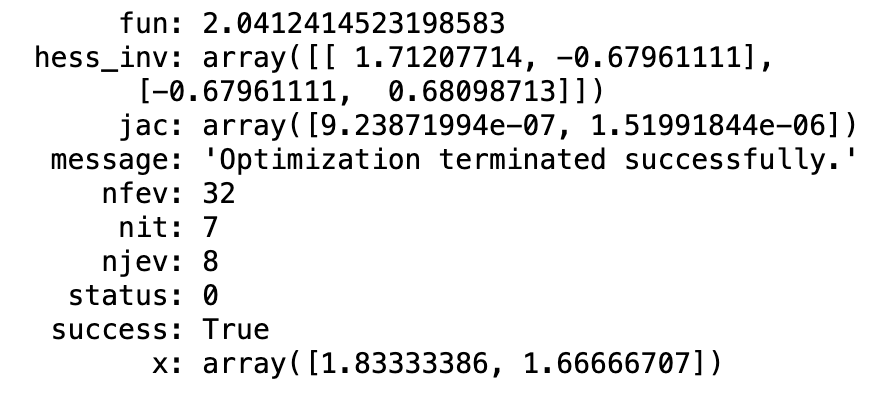
\includegraphics[scale = 0.4]{\pathtoimages/ex2-5.png}
\end{center}
\end{frame}

\begin{frame}
\frametitle{Extreme Value Theorem for Functions of Two Variables}
\begin{Theorem}
If $f$ is continuous on a closed and bounded set $D$ in $\mathbb{R}^2$, then $f$ attains an absolute maximum value $f(x_1, y_1)$ and an absolute minimum value $f(x_2, y_2)$ at some points $(x_1, y_1)$ and $(x_2, y_2)$ in $D$.
\end{Theorem}
\end{frame}

\begin{frame}[t]
\frametitle{Global Optimization}
\begin{Example}
Find the absolute maximum and minimum values of $f(x, y) = 5 - 3x + 4y$ on the triangular region with vertices $(0, 0)$, $(4, 0)$, $(4, 5)$.
\end{Example}
\end{frame}

\begin{frame}
\frametitle{Global Optimization in Python}
\tiny
There are many global optimization techniques in Python. However, they tend to be slow and not particularly effective on functions that aren't convex or concave. See the \href{https://docs.scipy.org/doc/scipy/reference/optimize.html}{SciPy documentation} for more details. 
\begin{center}
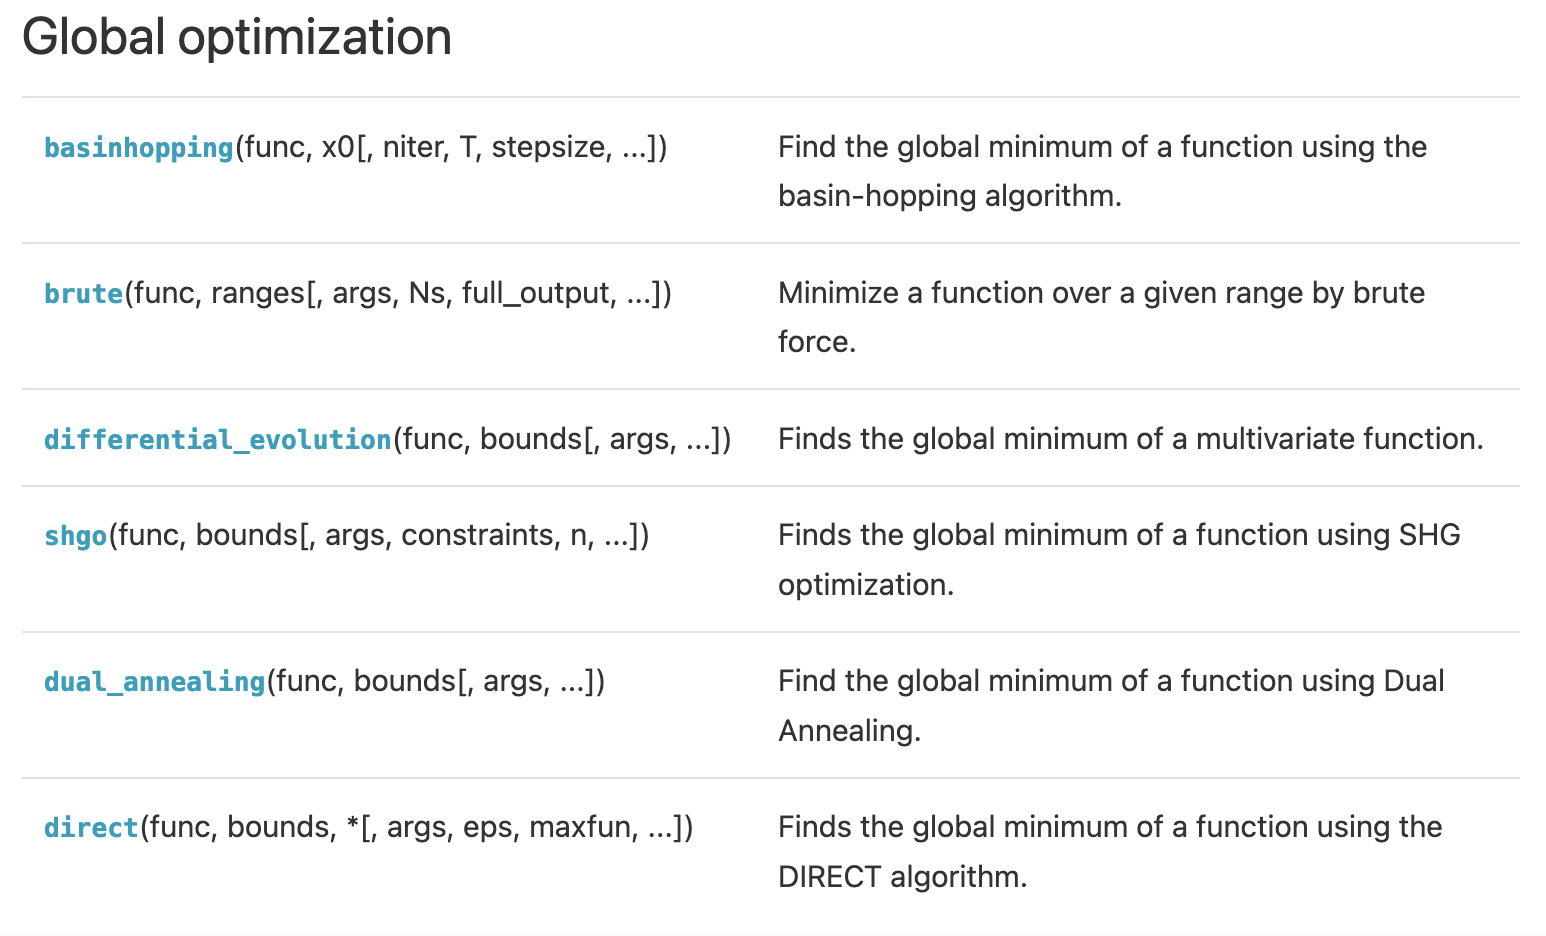
\includegraphics[scale = 0.3]{\pathtoimages/global.png}
\end{center}
\end{frame}

\begin{frame}
\frametitle{Lagrange Multipliers}
For ${\boldsymbol x}\in \mathbb{R}^n$, consider $f({\boldsymbol x})$ subject to $g({\boldsymbol x}) = k$. If local extrema exist, they satisfy the equation
$$
\nabla f({\boldsymbol x}) = \lambda \nabla g({\boldsymbol x}).
$$
for some $\lambda$ in $\mathbb{R}$.
\end{frame}


\begin{frame}
\frametitle{Lagrange Multipliers Picture}
\begin{center}
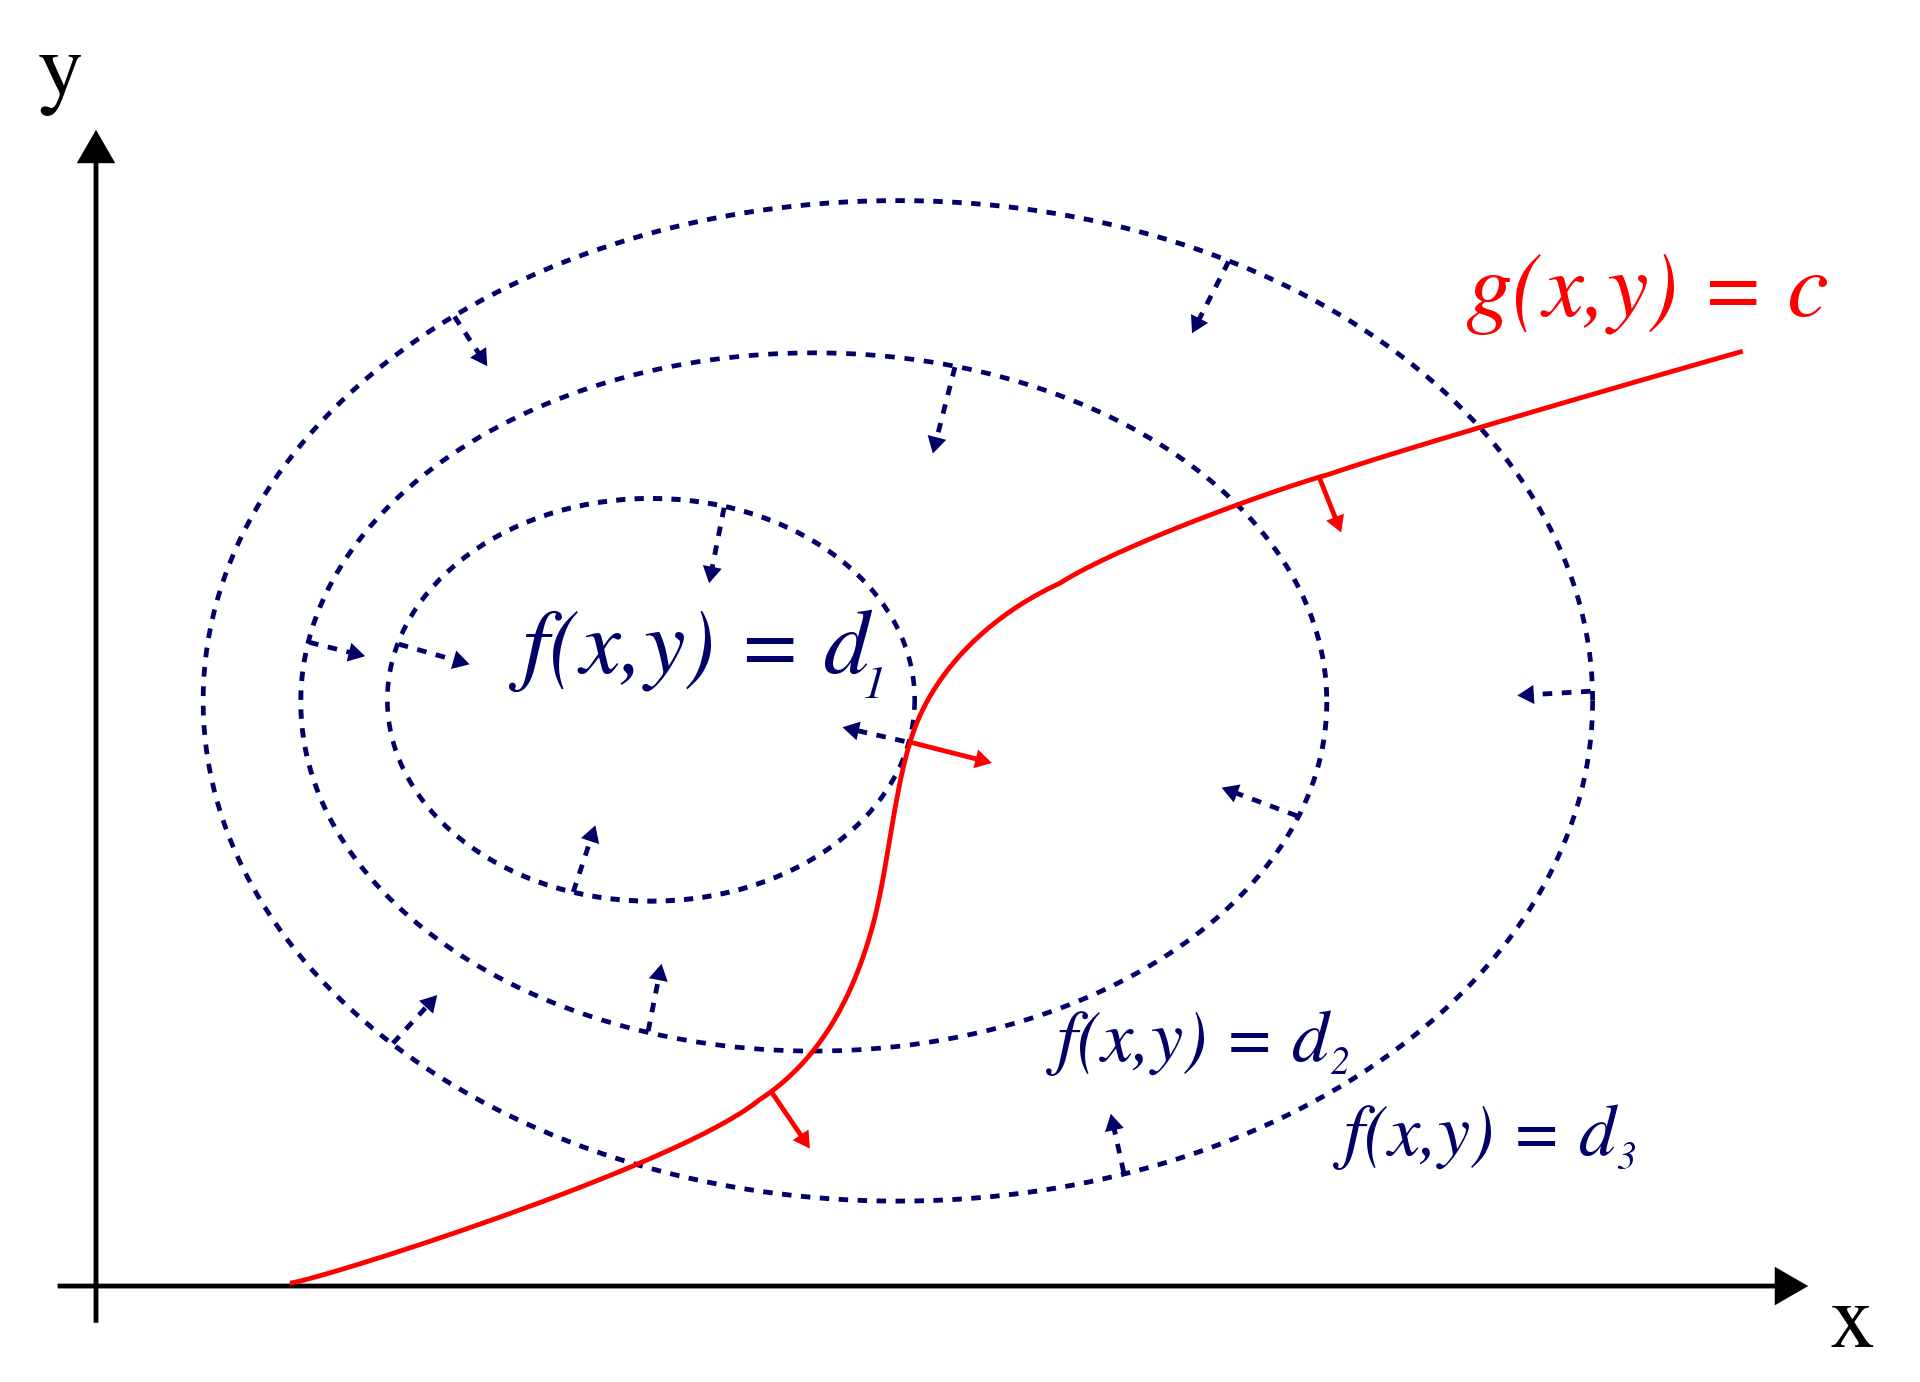
\includegraphics[scale = 0.1]{\pathtoimages/LagrangeMultipliers.png}
\end{center}
\end{frame}

\begin{frame}[t]
\frametitle{Lagrange Multipliers Example}
\begin{Example}
Find the shortest distance from the point $(1, 0, -2)$ to the plane $x + 2y + z = 4$.
\end{Example}
\end{frame}

\subsection{Multiple Integrals}

\begin{frame}
\frametitle{Construction of Double Integral}
\tiny
Consider $f:\mathbb{R}^2\to\mathbb{R}$ and define the closed region
$$
R = [a, b]\times [c, d] = \{(x, y)\in\mathbb{R}^2| a\leq x\leq b,\ c\leq y\leq d\}.
$$
Consider partition $P$ of $R$ into subrectangles $R_{ij} = [x_{i - 1}, x_i]\times [y_{i - 1}, y_i]$, where
\begin{align*}
a &= x_0 \leq x_1 < \ldots < x_m = b\\
c &= y_0 \leq y_1 < \ldots < y_n = d\\
\end{align*}
Select $(s_{ij}, t_{ij})$ from $R_{ij}$. The area of $R_{ij}$ is $\Delta A_{ij} = \Delta x_i\Delta y_j$. Define the mesh $\|P\| = \max\limits_{i, j}\{\Delta A_{ij}\}$. Then
$$
\iint_R f(x, y)\ dA = \lim_{\|P\|\to 0} \sum_{i = 1}^m\sum_{j = 1}^n f(s_{ij}, t_{ij})\ \Delta A_{ij}
$$
whenever the limit exists.
\end{frame}

\begin{frame}[t]
\frametitle{Double Integral Example}
\begin{Example}
Calculate $\displaystyle\iint_{[0,1]\times[0, 1]} xy^2\ dA$. Use a uniform partition with $n^2$ subrectangles $R_{ij}$, and the upper right point of $R_{ij}$ for $(s_{ij}, t_{ij})$.
\end{Example}
\end{frame}

\begin{frame}[fragile]
\frametitle{Double Integral Python Example}
\small
\begin{Example}
Use \texttt{scipy.integrate.dblquad} to verify the previous result for $\displaystyle\iint_{[0,1]\times[0, 1]} xy^2\ dA$.
\end{Example}
\begin{lstlisting}[language=Python]
# See https://docs.scipy.org/doc/scipy/reference/generated/scipy.integrate.dblquad.html
from scipy.integrate import dblquad

# Define f; integrate y the x
f = lambda y, x: x * y**2

# Integrate; integrate 3rd to 4th input then 2nd to 3rd input
dblquad(f, 0, 1, 0, 1)[0]
\end{lstlisting}
The output is \texttt{0.16666666666666669} which agrees with our previous result. 

\end{frame}

\begin{frame}
\frametitle{Fubini's Theorem}
\begin{Theorem}[Fubini]
Consider $R = [a, b]\times [c, d]$ and define
$$
A_1(x) = \int_c^d f(x, y)\ dy\qquad A_2(y) = \int_a^b f(x, y)\ dx.
$$
Then
$$
\iint_R f(x, y)\ da = \int_a^b A_1(x)\ dx = \int_c^d A_2(y)\ dy.
$$
\end{Theorem}
\end{frame}

\begin{frame}[t]
\frametitle{Fubini's Theorem Example}
\begin{Example}
Evaluate $\displaystyle\iint_R y\sin(xy)\ dA$, where $R = [1, 2]\times \left[0, \frac{\pi}{2}\right]$.
\end{Example}

\end{frame}

\begin{frame}
\frametitle{Integral over General Region}
Theoretically speaking, to calculate
$$
\iint_D f(x, y)\ dA
$$
where $D$ isn't a rectangle, simply choose rectangle $R$ which contains $D$ and define
$$
F(x, y) = \begin{cases} f(x, y),	&	(x, y)\in D\\ 0,	&	(x,y)\in R\setminus D.\end{cases}
$$
The next slide will help show how to handle these integrals in practice. 
\end{frame}

\begin{frame}[t]
\frametitle{Integral of General  Region}
\begin{Example}
Compute $\displaystyle\iint_D xy^2\ dA$, where $D$ is the triangular region with vertices $(0, 0)$, $(0, 2)$, and $(1, 0)$.
\end{Example}

\end{frame}

\subsection{Change of Variables}

\begin{frame}
\frametitle{Jacobian}
\begin{Definition}
The {\bf Jacobian} of the transformation given by $x = g(u, v)$ and $y = h(u, v)$ is
$$
J = \left(\begin{array}{c c} \frac{\partial x}{\partial u}	&	\frac{\partial x}{\partial v}\\ \frac{\partial y}{\partial u} &	\frac{\partial y}{\partial v}\end{array}\right).
$$
\end{Definition} 

\end{frame}

\begin{frame}
\frametitle{Change of Variables}
Suppose that we have a one-to-one transformation with continuous partial derivatives that maps the $uv$-plane to the $xy$-plane, and in particular the region $S$ to $D$. Then
$$
\iint_D f(x, y)\ dxdy = \iint_S f\left(x(u, v), y(u, v)\right)\left|\text{det}(J)\right|\ dudv.
$$

\end{frame}

\begin{frame}[t]
\frametitle{Change of Variables Example}
\begin{Example}
$\displaystyle\int_{-\infty}^{\infty} e^{-x^2/2}\ dx = $
\end{Example}

\end{frame}

\begin{frame}
\frametitle{Jacobian on YouTube}
\small
Watch the Mathemaniac video about the Jacobian on YouTube (\url{https://youtu.be/wCZ1VEmVjVo}).
\begin{center}

\includegraphics[scale = 0.3]{\pathtoimages/Mathemaniac.png}
\end{center}
\end{frame}

\end{document}
